\documentclass[cn,11pt]{elegantbook}
\usepackage{float}
\usepackage{tikz}
\usepackage{titlesec}
% \titleclass{\clearpage\section}{top}
% \newcommand\clearpage\sectionbreak{\clearpage}

\title{高中物理学讲义}
\subtitle{Elegant\LaTeX{} }

\author{Tylor Gan}
\institute{Tencent}
\date{\today}
\version{1989}

\extrainfo{So far as the theories of mathematics are about reality, they are not certain; 
so far as they are certain, they are not about reality. --- Albert Einstein}

\logo{logo.png}
\cover{cover.jpg}

\begin{document}

\maketitle

\tableofcontents

% \thispagestyle{empty}

\mainmatter
\hypersetup{pageanchor=true}
\chapter{描述运动的基本概念}
   \begin{enumerate}
      \item 质点
      \begin{itemize}
         \item 用来代替物体的有质量的点叫做质点.
         \item 研究一个物体的运动时,如果物体的形状和大小对所研究问题的影响可以忽略,就可以将该运动物体看做质点.
         \item 质点是一种理想化模型,实际并不存在.
      \end{itemize}
      \item 参考系
      \begin{itemize}
         \item 参考系可以是运动的物体,也可以是静止的物体,但被选为参考系的物体,我们都假定它是静止的.
         \item 选取不同的物体作为参考系,对同一物体运动的描述可能相同,也可能不同. 通常以地面为参考系.
      \end{itemize}
      \item 位移
      \begin{itemize}
         \item 定义:表示质点的位置变动,它是质点由初位置指向末位置的有向线段.
         \item 与路程的区别:位移是矢量,路程是标量. 只有在单向直线运动中,位移的大小才等于路程.   
      \end{itemize}
      \item 速度
      \begin{itemize}
         \item 物理意义:描述物体运动快慢和运动方向的物理量,是状态量.
         \item 定义式:$v=\frac{\Delta x}{\Delta t}$.
         \item 大小:在数值上等于单位时间内物体位移的大小.
         \item 方向:与位移同向,即物体运动的方向.
      \end{itemize}
      \item 平均速度
      \begin{itemize}
         \item 在变速运动中,物体在某段时间内的 位移与发生这段位移所用时间的比值叫做这段时间内的平均速度,即$\overline{v}=\frac{\Delta x}{\Delta t}$,其方向与位移的方向相同.
         \item 平均速度反映一段时间内物体运动的平均快慢程度,它与一段时间或一段位移相对应.
      \end{itemize}
      \item 瞬时速度
      \begin{itemize}
         \item 运动物体在某一时刻(或某一位置)的速度,方向沿轨迹上物体所在点的切线方向指向前进的一侧,是矢量. 瞬时速度的大小叫速率,是标量.
         \item 瞬时速度能精确描述物体运动的快慢,它是在运动时间$\Delta t \rightarrow 0$时的平均速度,与某一时刻或某一位置相对应.
         \item 平均速率是路程与时间的比值,它与平均速度的大小没有对应关系.
      \end{itemize}
      \item 速度变化量
      \begin{itemize}
         \item 物理意义:描述物体速度改变的物理量,是过程量.
         \item 定义式:
         
         $\Delta v=v-v_{0}$.
         \item 大小:$\Delta v$可以由v与$v_{0}$进行矢量运算得到,也可以由$\Delta v=a \Delta t$计算得到.
         \item 方向:可以用矢量图形来描述Δv的方向,如图甲、乙、丙所示,$\Delta v$的方向由初速度($v_{0}$)矢量的末端指向末速(v)矢量的末端.
      \end{itemize}
      \begin{figure}[htbp]
         \centering
         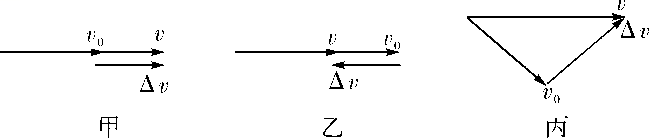
\includegraphics[width=0.8\textwidth]{11.png}
         \caption{速度变化量}
      \end{figure}

      \item 加速度
      \begin{itemize}
         \item 物理意义:描述物体速度变化快慢和变化方向的物理量,是状态量.
         \item 定义式:
         
         $a=\frac{\Delta v}{\Delta t}=\frac{v-v_{0}}{\Delta t}$.
         \item 决定因素:a不是由$v, \Delta t, \Delta v$来决定,而是由F、M来决定.
         \item 与$\Delta v$的方向一致,由合外力的方向决定,而与$v_{0}, v$的方向无关.
      \end{itemize}

   \end{enumerate}

   \clearpage\section{对质点概念的理解}
   \begin{example}
      在研究下述运动时,能把物体看做质点的是( B )

      A.研究短跑运动员的起跑动作时

      B.研究一架无人机的飞行快慢时

      C.将一枚硬币用力上抛并猜测它落地时正面是朝上还是朝下时

      D.研究汽车在上坡时有无翻倒的危险时
      \begin{solution}
         研究短跑运动员的起跑动作、抛出硬币落地时的上下面时,所研究对象的大小和形状不能忽略,故运动员和硬币都不能看做质点;研究汽车翻倒是转动问题,不能将汽车看做质点;研究飞机飞行快慢时,可把飞机看做质点.故选项B正确.

         
      \end{solution}
      
   \end{example}
   \begin{note}
      建立质点模型的两个关键点
      \begin{itemize}
         \item 明确题目中要研究的问题是什么.
         
         质点是对实际物体的科学抽象,是研究物体运动时对实际物体进行的近似,真正的质点并不存在.
         \item 分析物体的大小和形状对所研究的问题产生的影响能否忽略不计.
         
         当物体的大小和形状对所研究运动的影响很小,可以忽略不计时,就可将其视为质点.
      \end{itemize}
   \end{note}


   \clearpage\section{位移与路程的区别和联系}
      \begin{figure}[htbp]
         \centering
         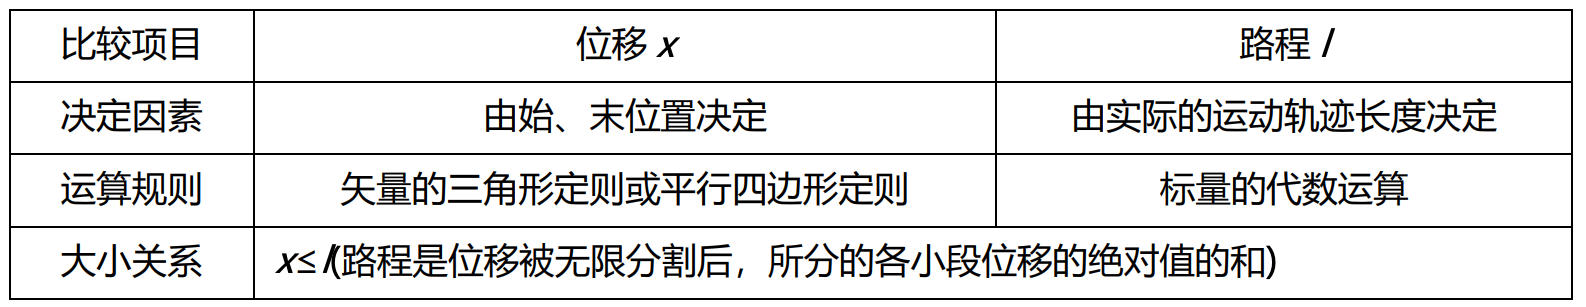
\includegraphics[width=0.8\textwidth]{t11.png}
      \end{figure}

      
      \begin{example}
         (2017·湖南株洲质检)(多选)关于位移和路程,下列说法正确的是( BD )

         A.物体在某一段时间内运动的位移为零,则其一定是静止的

         B.物体在某一段时间内运动的路程为零,则其一定是静止的

         C.在直线运动中,物体的位移大小一定等于其路程

         D.在曲线运动中,物体的位移大小一定小于路程
         \begin{solution}
            路程指物体运动轨迹的长度,而位移指由初位置指向末位置的有向线段,只有当物体做单向直线运动时,其位移大小才等于路程.容易判断选项B、D正确,A、C错误.

            
         \end{solution}

      
         
      \end{example}

   \clearpage\section{平均速度与瞬时速度的区别和联系}
   \begin{itemize}
      \item 两种物体的速度
      \begin{itemize}
         \item 瞬时速度是运动时间$\Delta t \rightarrow 0$时的平均速度.
         \item 对于匀速直线运动,瞬时速度与平均速度相等.
      \end{itemize}
      \item 关于用平均速度法求瞬时速度
      \begin{itemize}
         \item 方法概述:由平均速度公式$\overline{v}=\frac{\Delta x}{\Delta t}$可知,当$\Delta x、\Delta t$都非常小,趋向于极限时,这时的平均速度就可认为是某一时刻或某一位置的瞬时速度.
         \item 选用思路:当已知物体在微小时间$\Delta t$内发生的微小位移$\Delta x$时,可由$\overline{v}=\frac{\Delta x}{\Delta t}$粗略地求出物体在该位置的瞬时速度.
            
      \end{itemize}
   \end{itemize}
   \begin{example}
      (多选)如图1.2所示,物体沿曲线轨迹的箭头方向运动,AB、ABC、ABCD、ABCDE四段曲线轨迹运动所用的时间分别是1 s、2 s、3 s、4 s.下列说法正确的是( ABC )
      \begin{figure}[htbp]
         \centering
         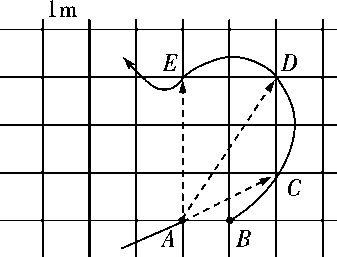
\includegraphics[width=0.2\textwidth]{12.png}
         \caption{}
      \end{figure}
   
      A.物体在AB段的平均速度大小为1 m/s
      
      B.物体在ABC段的平均速度大小为52 m/s
      
      C.AB段的平均速度比ABC段的平均速度更能反映物体处于A点时的瞬时速度
      
      D.物体在B点的速度等于AC段的平均速度
      \begin{solution}
         由$\overline{v}=\frac{\Delta x}{\Delta t}$可得$\overline{v}_{A B}=\frac{1}{1} \mathrm{m} / \mathrm{s}=1 \mathrm{m} / \mathrm{s}, \quad \overline{v}_{A C}=\frac{\sqrt{5}}{2} \mathrm{m} / \mathrm{s}$,故选项A、B均正确;所选取的过程离A点越近,其阶段的平均速度越接近A点的瞬时速度,故选项C正确;由A经B到C的过程不是匀变速直线运动过程,故B点虽为AC段的中间时刻,但其速度不等于AC段的平均速度,故选项D错误.
         
      \end{solution}
   
      
   \end{example}
   \begin{note}
      平均速度和瞬时速度的三点注意
      \begin{itemize}
         \item 求解平均速度必须明确是哪一段位移或哪一段时间内的平均速度.
         \item $\overline{v}=\frac{\Delta x}{\Delta t}$是平均速度的定义式,适用于所有的运动.
         \item 用平均速度法近似求解瞬时速度,不仅适用于直线运动,也适用于曲线运动.时间越短,平均速度越接近于瞬时速度.
      \end{itemize}
   \end{note}


   \clearpage\section{速度、速度的变化量和加速度的关系}

   \begin{itemize}
      \item 速度的大小与加速度的大小没有必然联系.
      \item 速度变化量与加速度没有必然的联系,速度变化量的大小由加速度和速度变化的时间决定.
      \item $a=\frac{\Delta v}{\Delta t}$是加速度的定义式;加速度的决定式是$a=\frac{F}{m}$,即加速度的大小由物体受到的合力F和物体的质量m共同决定,加速度的方向由合力的方向决定.
      \item 速度增大或减小由速度与加速度的方向关系决定
      \begin{figure}[htbp]
         \centering
         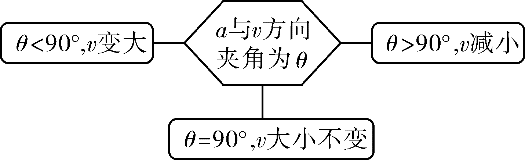
\includegraphics[width=0.4\textwidth]{13.png}
      \end{figure}
   
   \end{itemize}
   \begin{example}
      一质点在x轴上运动,初速度$v_{0}>0$,加速度$a>0$,当加速度a的值由零逐渐增大到某一值后再逐渐减小到零,则该质点( B )
      
      A.速度先增大后减小,直到加速度等于零为止
      
      B.速度一直在增大,直到加速度等于零为止
      
      C.位移先增大,后减小,直到加速度等于零为止
      
      D.位移一直在增大,直到加速度为0为止
      \begin{solution}
         由于加速度的方向始终与速度方向相同,质点速度逐渐增大,当加速度减小到零时,速度达到最大值,选项A错误,B正确;位移逐渐增大,当加速度减小到零时,速度不再变化,位移将随时间继续增大,选项C、D错误.

         
      \end{solution}
   
      
   \end{example}
   \begin{note}
      对加速度大小和方向的进一步理解
      \begin{figure}[htbp]
         \centering
         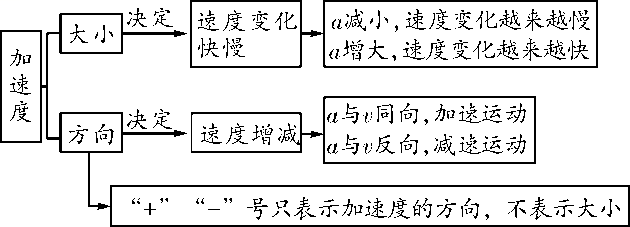
\includegraphics[width=0.5\textwidth]{14.png}
      \end{figure}

      
   \end{note}

   

\chapter{匀变速直线运动的规律及应用}
\begin{enumerate}
   \item 基本规律
   \begin{itemize}
      \item 速度公式:$v=v_{0}+a t$
      \item 位移公式:$x=v_{0} t+\frac{1}{2} a t^2$
      \item 位移速度关系式:$v^{2}-v_{0}^{2}=2 a x$
   \end{itemize}
   \item 两个重要推论
   \begin{itemize}
      \item 物体在一段时间内的平均速度等于这段时间中间时刻的瞬时速度,还等于初、末时刻速度矢量和的一半,即
      
      $v_{\frac{t}{2}}=\frac{v_{0}+v}{2}$.
      \item 任意两个连续相等的时间间隔T内的位移之差为一恒量,即
      
      $\Delta x=x_{2}-x_{1}=x_{3}-x_{2}=\ldots=x_{n}-x_{n-1}=a T^{2}$
   \end{itemize}
   \item $v_{0}=0$的四个重要推论
   \begin{itemize}
      \item 1T末、2T末、3T末……瞬时速度的比为
      
      $v_{1} : v_{2} : v_{3} : \ldots : v_{n}=1 : 2 : 3 : \ldots : n$..
      \item 1T内、2T内、3T内……位移的比为
      
      $x_{1} : x_{2} : x_{3} : \ldots : x_{0}=1^{2} : 2^{2} : 3^{2} : \ldots : n^{2}$.
      \item 第一个T内、第二个T内、第三个T内……位移的比为
      
      $x_{\mathrm{I}} : x_{\mathrm{II}} : x_{\mathrm{III}} : \ldots : x_{n}=1 : 3 : 5 : \ldots :(2 n-1)$.
      \item 从静止开始通过连续相等的位移所用时间的比为
      
      $t_{1} : t_{2} : t_{3} : \ldots : t_{n}=1 :(\sqrt{2}-1) :(\sqrt{3}-\sqrt{2}) : \ldots :(\sqrt{n}-\sqrt{n-1})$.  
   \end{itemize}
   \item 自由落体运动
   \begin{itemize}
      \item 条件:物体只受重力,从静止开始下落..
      \item 基本规律:
      \begin{itemize}
         \item 速度公式$v=g t$;
         \item 位移公式$h=\frac{1}{2} g t^{2}$;
         \item 速度位移关系式$v^{2}=2 g h$.
      \end{itemize}
   \end{itemize}
   \item 竖直上抛运动
   \begin{itemize}
      \item 运动特点:
      
      加速度为g,上升阶段做匀减速直线运动,下降阶段做自由落体运动.
      \item 基本规律:
      \begin{itemize}
         \item 速度公式$v=v_{0}-g t$;
         \item 位移公式$h=v_{0} t-\frac{1}{2} g t^{2}$;
         \item 速度位移关系式$v^{2}-v_{0}^{2}=-2 g h$.
      \end{itemize}
   \end{itemize}
\end{enumerate}

   \clearpage\section{匀变速直线运动的规律及应用}
   \begin{itemize}
      \item 运动学公式中正、负号的规定
      \begin{itemize}
         \item 除时间$t$外,$x, v_{0}, v, a$均为矢量,所以需要确定正方向,一般以$v_{0}$的方向为正方向.
         与初速度同向的物理量取正值,反向的物理量取负值,当$v_{0}=0$时,一般以加速度a的方向为正方向.
         \item 五个物理量$t, v_{0},  v,  a, x$必须针对同一过程.
      \end{itemize}
      \item 解决匀变速直线运动问题常用的“六法”
      
      \begin{figure}[htbp]
         \centering
         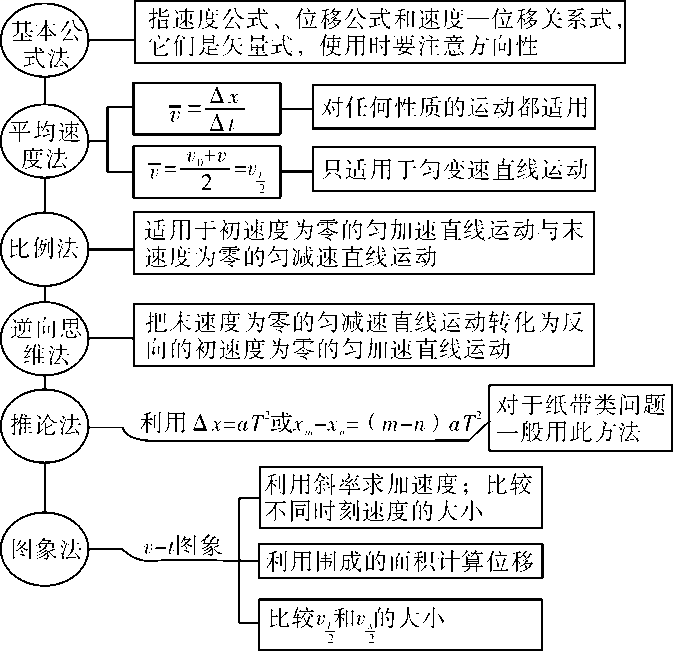
\includegraphics[width=0.5\textwidth]{15.png}
      \end{figure}

      \begin{example}
         (2017·湖南岳阳检测)如图所示,是冰壶以速度v垂直进入四个宽为l的矩形区域沿虚线做匀减速直线运动,且刚要离开第四个矩形区域的E点时速度恰好为零,冰壶通过前三个矩形的时间为t,试通过所学知识分析并计算冰壶通过第四个矩形所用的时间是多少?(可选用多种方法)
      
      \begin{figure}[htbp]
         \centering
         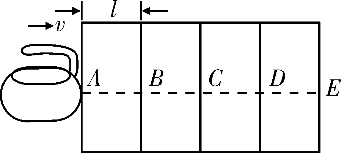
\includegraphics[width=0.2\textwidth]{16.png}
      \end{figure}
      
         \begin{solution}

            根据位移公式和速度公式,由A到E,有
            $4 l=v t_{1}-\frac{1}{2} a t^{2}, \quad 0=v-a t_{1}$,
            式中,$t_{1}$为冰壶通过四个矩形区域所用的时间,a为其加速度的大小,
            由A到D,有$3 l=v t-\frac{1}{2} a t^{2}$,
            联立解得$t_{1}=2 t$或$t_{1}=\frac{2}{3} t$,
            显然$t_{1}=\frac{2}{3} t$不符合题意,应舍去.
            所以冰壶通过第四个矩形所用的时间为$t^{\prime}=t_{1}-t=t$.

            答案  t

            
         \end{solution}   
         
      \end{example}
      \begin{note}
         求解匀变速直线运动问题的基本思路
               
      \begin{figure}[H]
         \centering
         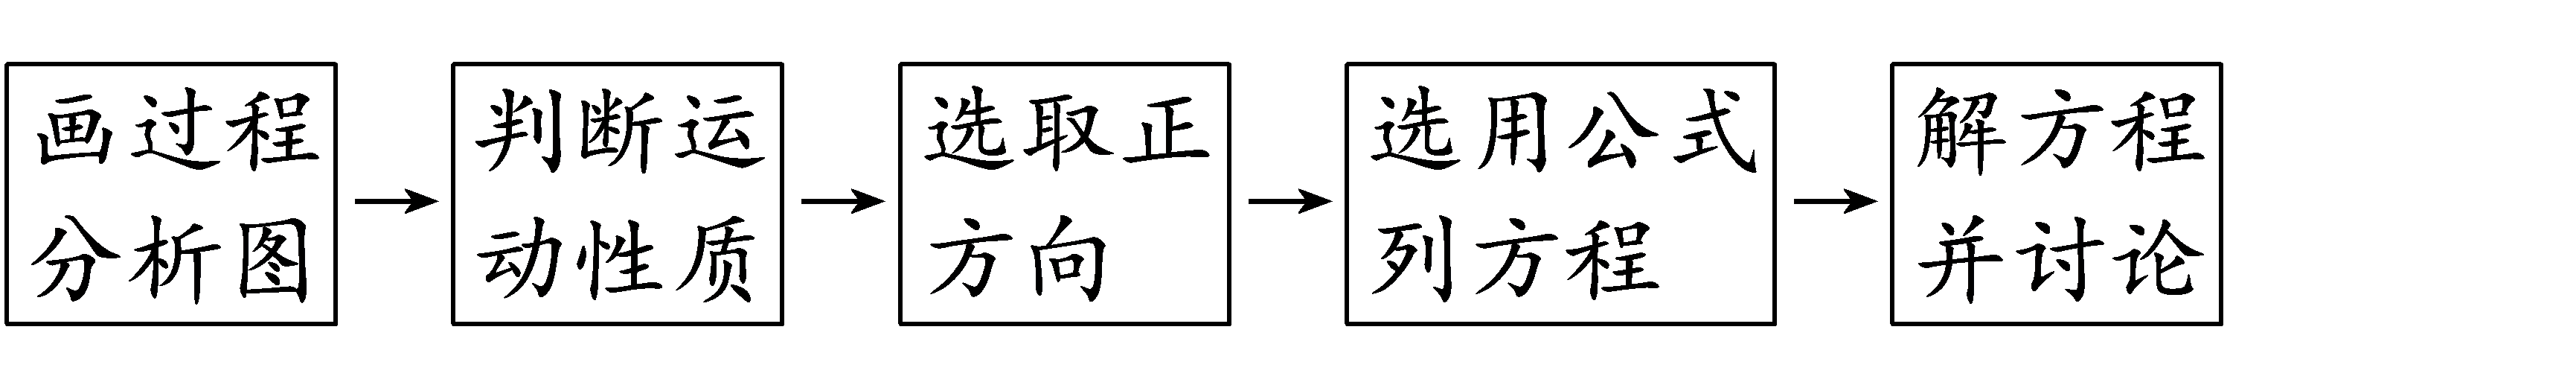
\includegraphics[width=0.7\textwidth]{17.png}
      \end{figure}
      

      \end{note}
   \end{itemize}

   \clearpage\section{自由落体和竖直上抛运动的分析}
   \begin{example}
      (2017·山东济南调研)如图所示是一种较精确测量重力加速度g值的方法:将下端装有弹射装置的真空玻璃直管竖直放置,玻璃管足够长,小球竖直向上被弹出,在O点与弹簧分离,然后返回,在O点正上方选取一点P,利用仪器精确测得OP间的距离为H,从O点出发至返回O点的时间间隔为T1,小球两次经过P点的时间间隔为T2.求:
      
      (1)重力加速度g;
      
      (2)若O点距玻璃管底部的距离为L0,求玻璃管最小长度.
   \begin{solution}
      (1)小球从O点上升到最高点有$h_{1}=\frac{1}{2} g\left(\frac{T_{1}}{2}\right)^{2}$
      ,小球从P点上升到最高点有$h_{2}=\frac{1}{2} g\left(\frac{T_{2}}{2}\right)$
      ,依据题意有$h_{1}-h_{2}=H$,联立解得$g=\frac{8 H}{T_{1}^{2}-T_{2}^{2}}$.
      
      (2)真空管最小长度$L=L_{0}+h_{1}$,解得$L=L_{0}+\frac{T_{1}^{2} H}{T_{1}^{2}-T_{2}^{2}}$.
      
      答案 

      (1)$\frac{8 H}{T_{1}^{2}-T_{2}^{2}}$ 
      
      (2)$L_{0}+\frac{T_{1}^{2} H}{T_{1}^{2}-T_{2}^{2}}$
   \end{solution}   
   \end{example}
   \begin{note}
      竖直上抛运动的分析方法
      \begin{itemize}
         \item 分段法:可以把竖直上抛运动分成上升阶段的匀减速运动和下降阶段的自由落体运动处理,下降过程是上升过程的逆过程.
         \item 整体法:从全过程来看,加速度方向始终与初速度的方向相反,所以也把竖直上抛运动看成是一个匀变速直线运动.
      \end{itemize}
      
   \end{note}

   

\chapter{运动图象追及和相遇问题}
\begin{enumerate}
   \item 直线运动的x-t图象
   \begin{itemize}
      \item 意义:反映了直线运动的物体位移随时间变化的规律.
      \item 图线上某点切线的斜率的意义
      \begin{itemize}
         \item 斜率大小:表示物体速度的大小
         \item 斜率的正负:表示物体速度的方向
      \end{itemize}
      \item 两种特殊的x-t图象
      \begin{itemize}
         \item 若x-t图象是一条平行于时间轴的直线,说明物体处于静止状态. (如图所示甲图线)
         \item 若x-t图象是一条倾斜的直线,说明物体在做匀速直线运动. (如图所示乙图线)
      \end{itemize}
   \end{itemize}
   \item 直线运动的v-t图象
   \begin{itemize}
      \item 意义:反映了直线运动的物体速度随时间变化的规律.
      \item 图线上某点切线的斜率的意义.
      \begin{itemize}
         \item 斜率的大小:表示物体加速度的大小
         \item 斜率的正负:表示物体加速度的方向
      \end{itemize}
      \item 两种特殊的v-t图象
      \begin{itemize}
         \item 匀速直线运动的v-t图象是与横轴平行的直线. (如图所示甲图线)
         \item 匀变速直线运动的v-t图象是一条倾斜的直线. (如图所示乙图线)
      \end{itemize}
      \item 图线与坐标轴围成的“面积”的意义
      \begin{itemize}
         \item 图线与坐标轴围成的“面积”表示相应时间内的位移.
         \item 若此面积在时间轴的上方,表示这段时间内的位移方向为正方向;若此面积在时间轴的下方,表示这段时间内的位移方向为负方向.
      \end{itemize}
   \end{itemize}
   \item 追及和相遇问题
   \begin{itemize}
      \item 两类追及问题.
      \begin{itemize}
         \item 若后者能追上前者,追上时,两者处于同一位置,且后者速度一定不小于前者速度.
         \item 若追不上前者,则当后者速度与前者相等时,两者相距最近            
      \end{itemize}
      \item 两类相遇问题
      \begin{itemize}
         \item 同向运动的两物体追及,追上时即相遇
         \item 相向运动的物体,当各自发生的位移大小之和等于开始时两物体间的距离时即相遇
         
      \end{itemize}
   \end{itemize}
\end{enumerate}

   \clearpage\section{x-t图象与v-t图象的区别}
   \begin{figure}[H]
      \centering
      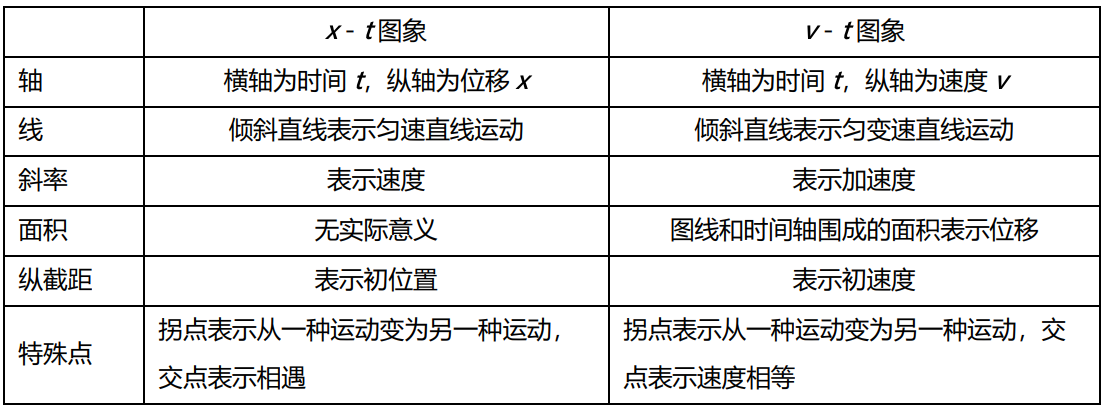
\includegraphics[width=1\textwidth]{t12.png}
   \end{figure}
   \begin{example}
      (2018·陕西汉中期末)在平直的公路上行驶的a车和b车,其位移—时间图象分别为图中直线a和曲线b,已知b车的加速度恒定且ab=-2 $m/s^{2}$,当t=3 s时,直线a和曲线b刚好相切,求t=0 s时a车和b车的距离x0.      

      \begin{figure}[htbp]
      \centering
      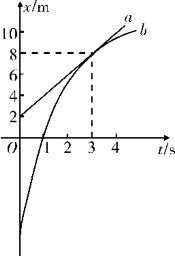
\includegraphics[width=0.2\textwidth]{19.png}
   \end{figure}

      \begin{solution}
         答案 9m
         
      \end{solution}   
      
   \end{example}
   \begin{note}
      运动图象中的易错点
      \begin{itemize}
         \item 对x-t图象,图线在纵轴上的截距表示t=0时物体的位置,对v-t或a-t图象,图线在纵轴上的截距并不表示t=0时物体的位置.
         \item 在v-t图象中,两条图线的交点不表示两物体相遇,而是表示两者速度相同.
         \item 两条图线在v轴上的截距不同,不少同学误认为两物体的初始位置不同,位置是否相同应根据题中条件确定.
      \end{itemize}
      
   \end{note}

   \clearpage\section{追及、相遇问题}
   讨论追及、相遇的问题,其实质就是分析讨论两物体在同一时刻能否到达相同的空间位置问题.
   \begin{itemize}
      \item 抓住一个条件,两个关系
      \begin{itemize}
         \item 一个条件:即两者速度相等,它往往是物体间能否追上、追不上或(两者)距离最大、最小的临界条件,也是分析判断的切入点.
         \item 两个关系:即时间关系和位移关系,这两个关系可通过画运动示意图得到.
      \end{itemize}
      \item 能否追上的判断方法
      
      常见情形:物体A追物体B,开始二者相距$x_{0}$,则
      \begin{itemize}
         \item A追上B时,必有$x_{A}-x_{B}=x_{0}$,且$v_{A} \geq v_{B}$.
         \begin{figure}[htbp]
            \centering
            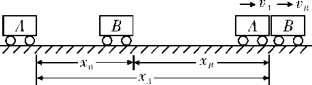
\includegraphics[width=0.5\textwidth]{110.png}
         \end{figure}

         \item 要使两物体恰好不相撞,必有$x_{A}-x_{B}=x_{0}$,$v_{A} = v_{B}$.
      \end{itemize}
      
   \end{itemize}
   \begin{example}
      (2018·江苏镇江模拟)甲、乙两车在同一直线轨道上同向行驶,
      甲车在前,速度为$v_{1}=8 \mathrm{m} / \mathrm{s}$,乙车在后,速度为$v_{2}=16m/s$,
      当两车相距$x_{0}=8 \mathrm{m}$时,甲车因故开始刹车,
      加速度大小为$a_{1}=2 \mathrm{m} / \mathrm{s}^{2}$,为避免相撞,
      乙车立即开始刹车,则乙车的加速度至少为多大?         

      \begin{solution}

         答案 6 $\mathrm{m} / \mathrm{s}^{2}$               
      \end{solution}   
      
   \end{example}

   \begin{note}
      追及和相遇问题的求解方法
      \begin{itemize}
         \item 解题思路
         \begin{figure}[htbp]
            \centering
            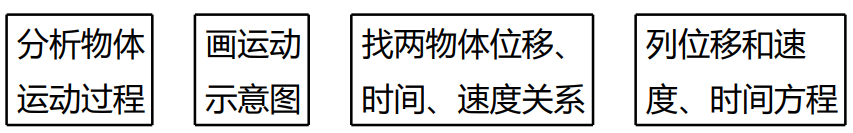
\includegraphics[width=0.5\textwidth]{111.png}
         \end{figure}

         \item 解题技巧
         \begin{itemize}
            \item 紧抓“一图三式”,即:过程示意图,时间关系式、速度关系式和位移关系式.
            \item 审题应抓住题目中的关键字眼,充分挖掘题目中的隐含条件.如“刚好”“恰好”“最多”“至少”等.往往对应一个临界状态,满足相应的临界条件.
            \item 若被追赶的物体做匀减速运动,一定要注意追上前该物体是否已经停止运动,另外还要注意最后对解的讨论分析.
         \end{itemize}
      \end{itemize}
      
   \end{note}



\chapter{重力 弹力 摩擦力}
   \begin{enumerate}
      \item 重力
      \begin{itemize}
         \item 产生:由于地球的吸引而使物体受到的力
         \item 大小:与物体的质量成正比,即$G=m g$.可用弹簧测力计测量重力.
         \item 方向:总是竖直向下的
         \item 重心:其位置与物体的质量分布和形状有关
         
      \end{itemize}
      \item 弹力
      \begin{itemize}
         \item 定义:发生弹性形变的物体由于要恢复原状而对与它接触的物体产生的作用力
         \item 产生的条件
         \begin{itemize}
            \item 物体间直接接触;
            \item 接触处发生弹性形变
            
         \end{itemize}
         \item 方向:总是与物体形变的方向相反
         
      \end{itemize}
      \item 胡克定律
      \begin{itemize}
         \item 内容:在弹性限度内,弹力的大小跟弹簧伸长(或缩短)的长度x成正比.
         \item 表达式:$F=k x$.$k$是弹簧的劲度系数,由弹簧自身的性质决定,单位是牛顿每米,用符号$\mathrm{N} / \mathrm{m}$表示. $x$是弹簧长度的变化量,不是弹簧形变以后的长度.
         
      \end{itemize}
      \item 滑动摩擦力和静摩擦力的对比
      \begin{figure}[htbp]
         \centering
         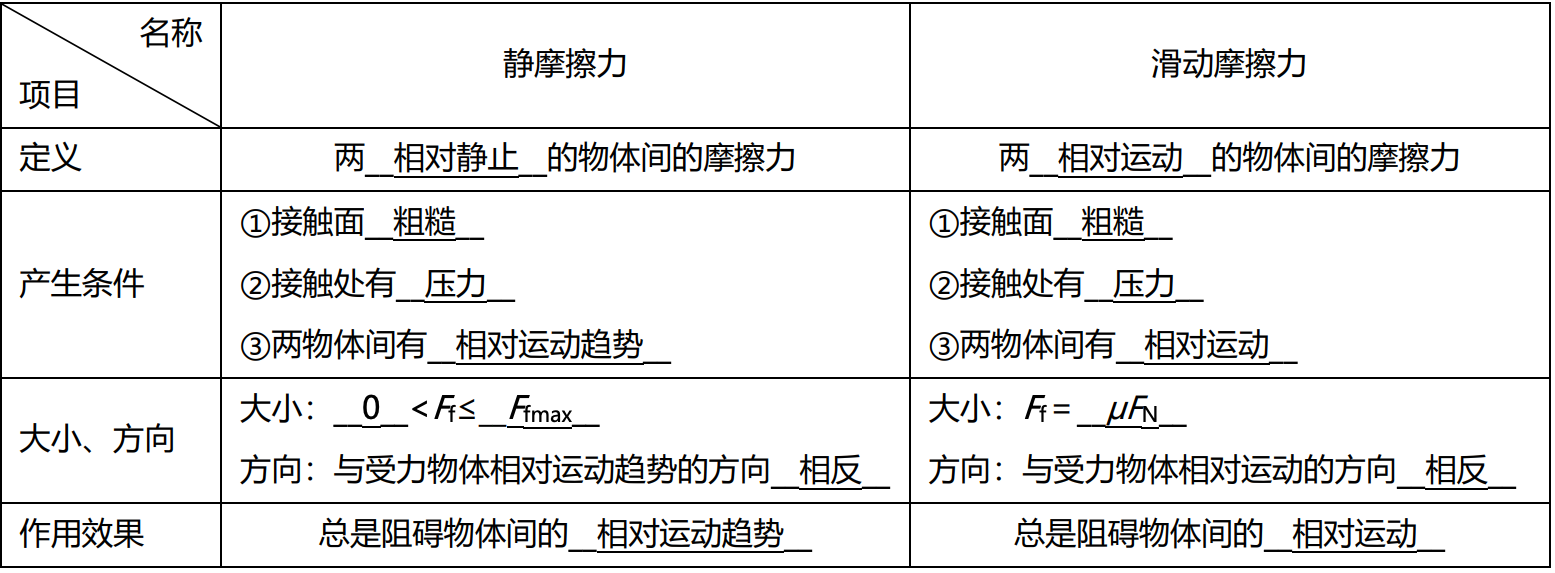
\includegraphics[width=1\textwidth]{t14.png}
      \end{figure}
      
      滑动摩擦力大小的计算公式$F_{\mathrm{f}}=\mu F_{\mathrm{N}}$中$μ$为比例常数,称为动摩擦因数,其大小与两个物体的材料和接触面的粗糙程度有关.
   \end{enumerate}

   \clearpage\section{弹力有无的判断}
   \begin{figure}[H]
      \centering
      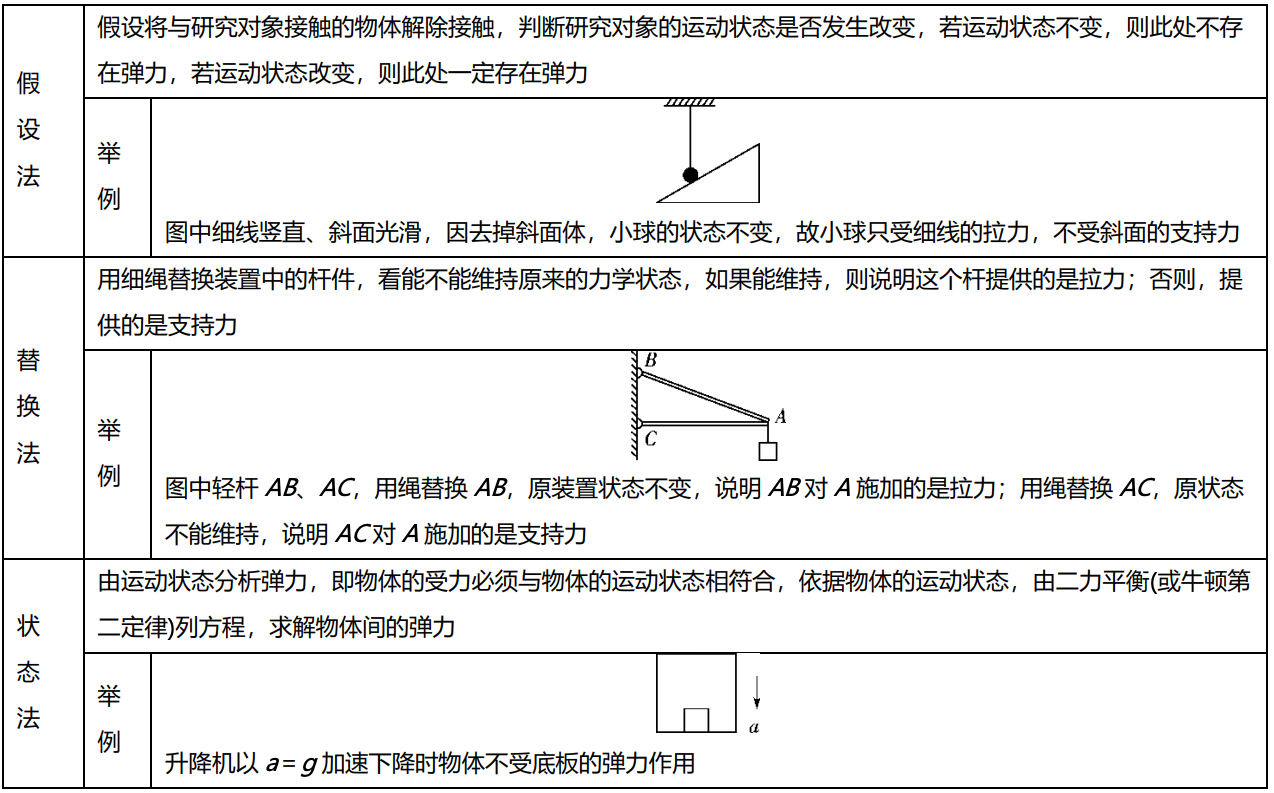
\includegraphics[width=1\textwidth]{t13.png}
   \end{figure}

   \begin{example}
      (2017·陕西西安调研)如图所示,在一个正方体的盒子中放有一个质量
      分布均匀的小球,小球的直径恰好和盒子内表面正方体的棱长相等,
      盒子沿倾角为α的固定斜面滑动,不计一切摩擦,
      下列说法中正确的是( A )         
      \begin{figure}[H]
      \centering
      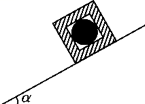
\includegraphics[width=0.3\textwidth]{21.png}
   \end{figure}
   
      \begin{solution}
         先以盒子和小球组成的系统为研究对象,无论上滑还是下滑,
         用牛顿第二定律均可求得系统的加速度大小为$a=g \sin \alpha$,
         方向沿斜面向下,由于盒子和小球始终保持相对静止,
         所以小球的加速度大小也是$a=g \sin \alpha$,方向沿斜面向下,
         小球沿斜面向下的重力分力大小恰好等于所需的合外力,
         因此不需要盒子的左、右侧面提供弹力.故选项A正确.               
      \end{solution}   
      
   \end{example}
   \begin{note}
      对于形变明显的物体,由形变情况直接判断弹力情况,对于形变不明显的物体通常用“假设法”和“替换法”,有时要根据物体的运动状态判定弹力情况.

      
   \end{note}

   \clearpage\section{弹力方向的确定和大小的计算}
   \begin{itemize}
      \item 弹力方向的确定
      \begin{figure}[H]
         \centering
         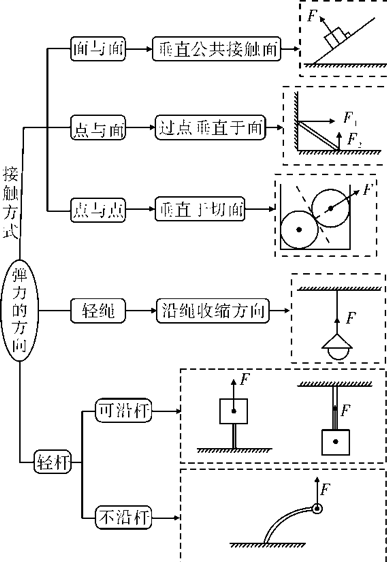
\includegraphics[width=0.5\textwidth]{t15.png}
      \end{figure}

      \item 计算弹力大小的三种方法
      \begin{itemize}
         \item 根据胡克定律进行求解
         \item 根据力的平衡条件进行求解
         \item 根据牛顿第二定律进行求解
      \end{itemize}

   \end{itemize}

   

   \begin{example}
      如图所示,固定在小车支架上的斜杆与竖直杆的夹角为$\theta$,
      在斜杆下端固定一个质量为m的小球,
      下列关于杆对球的作用力F的判断中正确的是( D )    
      
      A.小车静止时,$F=m g \cos \theta$,方向沿杆向上
      
      B.小车静止时,$F=m g \cos \theta$,方向垂直杆向上

      C.小车向右以加速度a运动时,一定有$F=\frac{m g}{\sin \theta}$

      D.小车向左以加速度a运动时,$F=\sqrt{(m a)^{2}+(m g)^{2}}$,
      方向斜向左上方,与竖直方向的夹角为α满足$\tan \alpha=\frac{a}{g}$

      \begin{figure}[H]
         \centering
         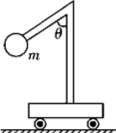
\includegraphics[width=0.2\textwidth]{112.png}
      \end{figure}
   
      \begin{solution}
         先以盒子和小球组成的系统为研究对象,无论上滑还是下滑,
         用牛顿第二定律均可求得系统的加速度大小为$a=g \sin \alpha$,
         方向沿斜面向下,由于盒子和小球始终保持相对静止,
         所以小球的加速度大小也是$a=g \sin \alpha$,方向沿斜面向下,
         小球沿斜面向下的重力分力大小恰好等于所需的合外力,
         因此不需要盒子的左、右侧面提供弹力.故选项A正确.               
      \end{solution}   
      
   \end{example}

   \begin{example}
      缓冲装置可抽象成如图所示的简单模型,图中A、B为原长相等、
      劲度系数分别为$k_{1}, k_{2}\left(k_{1} \neq k_{2}\right)$的两个不同的轻质弹簧.
      下列表述正确的是( D )
      \begin{figure}[H]
         \centering
         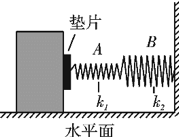
\includegraphics[width=0.2\textwidth]{113.png}
      \end{figure}
   
      A.装置的缓冲效果与两弹簧的劲度系数无关

      B.垫片向右移动稳定后,两弹簧产生的弹力之比$F_{1} : F_{2}=k_{1} : k_{2}$ 

      C.垫片向右移动稳定后,两弹簧的长度之比$I_{1} : l_{2}=k_{2} : k_{1}$

      D.垫片向右移动稳定后,两弹簧的压缩量之比$x_{1} : x_{2}=k_{2} : k_{1}$ 

      
   \end{example}

   \clearpage\section{静摩擦力的大小和方向}
   \begin{itemize}
      \item 静摩擦力有无的判断
      \begin{itemize}
         \item 假设法
         静摩擦力的方向一定与物体相对运动趋势的方向相反,利用“假设法”可以判断出物体相对运动趋势的方向.
         假设法(如图所示)
                        
         \begin{figure}[htbp]
            \centering
            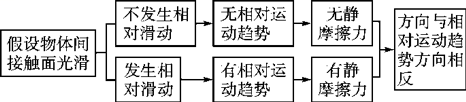
\includegraphics[width=0.3\textwidth]{t16.png}
         \end{figure}

         \item 状态法
         
         此法关键是先判明物体的运动状态(即加速度的方向),再利用牛顿第二定律(F=ma)确定合力,
         然后通过受力分析确定静摩擦力的大小及方向.
         \item 牛顿第三定律法
         
         此法的关键是抓住“力是物体间的相互作用”,
         先确定受力较少的物体受到的静摩擦力的方向,
         再根据“力的相互性”确定另一物体受到的静摩擦力方向.
      \end{itemize}
      \item 静摩擦力的计算方法
      \begin{itemize}
         \item 最大静摩擦力$F_{\mathrm{fmax}}$的计算
         最大静摩擦力$F_{\mathrm{fmax}}$只在刚好要发生相对滑动这一特定状态下才表现出来.
         比滑动摩擦力稍大些,
         通常认为二者相等,即$F_{\max }=\mu F_{N}$. 
         \item 一般静摩擦力的计算
         一般静摩擦力F的大小和方向都与产生相对运动趋势的力密切相关,
         跟接触面间相互挤压的弹力$F_{\mathrm{N}}$无直接关系,因此具有大小、方向的可变性.对具体问题要结合研究对象的运动状态(静止、匀速运动或加速运动),
         利用平衡条件或牛顿运动定律列方程求解.
      \end{itemize}
   \end{itemize}
   \begin{example}
      (2018·宁夏银川检测)指明物体A在以下四种情况下所受的静摩擦力的方向.
      \begin{figure}[htbp]
         \centering
         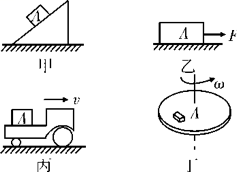
\includegraphics[width=0.2\textwidth]{114.png}
      \end{figure}
   
      (1)物体A静止于斜面上,如图甲所示;

      (2)物体A受到水平拉力F作用而仍静止在水平面上,如图乙所示;

      (3)物体A放在车上,在刹车过程中A相对于车厢静止,如图丙所示;

      (4)物体A在水平转台上,随转台一起匀速运动,如图丁所示.
      
      
   \end{example}
   \begin{note}
      应用“状态法”解题时应注意的问题

      状态法是分析判断静摩擦力有无及方向、大小的常用方法,在使用状态法处理问题时,需注意以下两点:
      \begin{itemize}
         \item 明确物体的运动状态,分析物体的受力情况,根据平衡方程或牛顿定律求解静摩擦力的大小和方向.
         \item 静摩擦力的方向与物体的运动方向没有必然关系,可能相同,也可能相反,还可能成一定的夹角.
      \end{itemize}
      
   \end{note}

   \clearpage\section{滑动摩擦力的大小和方向}
   \begin{itemize}
      \item 产生的条件
      \begin{itemize}
         \item 两物体相互接触且挤压,发生形变,产生弹力.
         \item 两接触面粗糙.
         \item 两物体沿接触面发生相对运动.
         
         以上三个条件必须同时具备,才会有滑动摩擦力存在.
      \end{itemize}
      \item 在计算滑动摩擦力的公式$F_{f}=\mu F_{N}$中,μ为动摩擦因数,
      其大小与接触面的材料、表面的粗糙程度有关;$F_{\mathrm{N}}$为两接触面间的正压力,其大小不一定等于物体的重力.
      \item 滑动摩擦力的大小与物体的运动速度无关,与接触面积也无关.
      \item 滑动摩擦力的方向总是与物体间相对运动的方向相反,但不一定与物体运动方向相反.

   \end{itemize}

   \begin{example}
      (2017·吉林长春检测)如图所示,质量为m的工件置于水平放置的钢板C上,
      二者间动摩擦因数为μ,由于固定的光滑导槽A、B的控制,工件只能沿水平导槽运动,
      现使钢板以速度$v_{1}$向右运动,
      同时用F拉动工件(F方向与导槽平行)使其以速度$v_{2}$沿导槽运动,则F的大小为( C )  
      \begin{figure}[htbp]
         \centering
         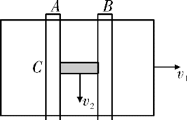
\includegraphics[width=0.2\textwidth]{115.png}
      \end{figure}
   
      A.等于μmg	
      
      B.大于μmg

      C.小于μmg	
      
      D.不能确定

      \begin{solution}
         钢板以速度$v_{1}$向右运动,则工件以等大速度相对钢板向左移动,设为$v_{1}$,
         同时工件被拉动也具有另一速度$v_{2}$,
         故工件相对于钢板的运动速度应是$v_{1}$与$v_{2}$的合成,即如上图中的速度v.滑动摩擦力阻碍二者的相对运动,故工件所受摩擦力$F_{f}$与$v$方向相反,
         要使工件沿导槽匀速运动,所施加的拉力只需与$F_{f}$一个分力平衡,
         故$F<F_{f} = μmg$.
         \begin{figure}[htbp]
            \centering
            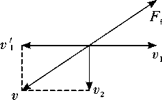
\includegraphics[width=0.2\textwidth]{116.png}
         \end{figure}

      \end{solution}
                  
      
   \end{example}

   \clearpage\section{摩擦力突变问题}
   \begin{note}
      解决摩擦力突变问题的关键点

      物体受到的外力发生变化时,
      物体受到的摩擦力的种类就有可能发生突变.
      解决这类问题的关键是:正确对物体受力分析和运动状态分析,
      从而找到物体摩擦力的突变“临界点”.
      
      常见类型如下:

      \begin{itemize}
         \item 静—静“突变”
         
         当作用在物体上的其他力的合力发生变化时,
         物体仍保持静止,而所受静摩擦力方向发生$180^{\circ}$“突变”,则“突变”点是静摩擦力为零时.
         \item 动—动“突变”
         
         某物体相对于另一物体滑动的过程中,若相对运动方向变了,
         则滑动摩擦力方向发生“突变”,“突变”点为两物体相对速度为零时.
         \item 静—动“突变”
         
         物体在摩擦力和其他力作用下处于静止状态,当其他力变化时,如果物体不能保持静止状态,
         则物体受到的静摩擦力将“突变”成滑动摩擦力,“突变”点为静摩擦力达到最大值时.
         \item 动—静“突变”
         
         两物体相对减速滑动的过程中,若相对速度变为零,
         则滑动摩擦力“突变”为静摩擦力,“突变”点为两物体相对速度刚好为零时.
      \end{itemize}
      
   \end{note}

   \begin{example}
      (多选)如图所示,将两相同的木块a、b置于粗糙的水平地面上,
      中间用一轻弹簧连接,两侧用细绳系于墙壁.开始时a、b均静止,弹簧处于伸长状态,
      两细绳均有拉力,a所受摩擦力$F_{fa}\neq0$,b所受摩擦力$F_{fb}=0$.
      现将右侧细绳剪断,则剪断瞬间( AD )   

      \begin{figure}[H]
         \centering
         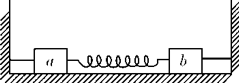
\includegraphics[width=0.3\textwidth]{117.png}
      \end{figure}
   
      A.$F_{fa}$大小不变	
      
      B.$F_{fa}$方向改变

      C.$F_{fb}$仍然为零	
      
      D.$F_{fb}$方向向右
      
                  
      
   \end{example}

   

   \begin{example}
      传送带以恒定的速率$v=10 m/s$运动,
      已知它与水平面成$\alpha=37^{\circ}$,如图所示,$PQ=16 m$,
      将一个小物体无初速度地放在P点,小物体与传送带间的动摩擦因数为$\mu=0.5$,
      问当传送带逆时针转动时,
      小物体运动到Q点的时间为多少?
      ($cos 37^{\circ}=0.8,sin 37^{\circ}=0.6$,g取$10 m/s^{2}$)

      \begin{figure}[H]
         \centering
         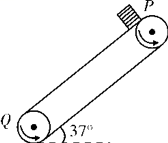
\includegraphics[width=0.2\textwidth]{118.png}
      \end{figure}
   
      \begin{solution}
         答案 2 s   
      \end{solution}
                  
      
   \end{example}

   \begin{note}
      摩擦力突变问题的分析步骤
      \begin{figure}[H]
         \centering
         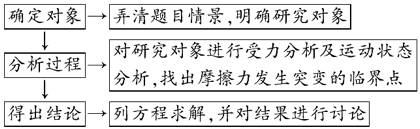
\includegraphics[width=0.6\textwidth]{t17.png}
      \end{figure}

      
   \end{note}



\chapter{力的合成与分解}
   \begin{enumerate}
      \item 力的合成
      \begin{itemize}
         \item 合力与分力
         \begin{itemize}
            \item 定义:如果几个力共同作用产生的效果与一个力的作用效果相同,这一个力就叫做那几个力的合力,那几个力叫做这一个力的分力
            \item 关系:合力与分力是等效替代关系
            
         \end{itemize}
         \item 共点力:作用在物体的同一点,或作用线的延长线交于一点的几个力
         \item 力的合成
         \begin{itemize}
            \item 定义:求几个力的合力的过程
            \item 运算法则
            \begin{itemize}
               \item 平行四边形定则:求两个互成角度的共点力的合力,可以用表示这两个力的线段为邻边作平行四边形,这两个邻边之间的对角线就表示合力的大小和方向(图甲).
               \item 三角形定则:把两个矢量的首尾顺次连接起来,第一个矢量的首到第二个矢量的尾的有向线段为合矢量(图乙).
               
            \end{itemize}
            
         \end{itemize}
         
      \end{itemize}
      \item 力的分解
      \begin{itemize}
         \item 定义:求一个力的分力的过程,力的分解是力的合成的逆运算
         \item 遵循的原则
         \begin{itemize}
            \item 平行四边形定则
            \item 三角形定则
            
         \end{itemize}
         \item 分解方法
         \begin{itemize}
            \item 力的作用效果分解法
            \item 正交分解法
            
         \end{itemize}
         
      \end{itemize}
      \item 矢量和标量
      \begin{itemize}
         \item 矢量
         
         既有大小又有方向的物理量,相加时遵循平行四边形定则. 如速度、力等.
            
         \item 标量
         
         只有大小没有方向的物理量,求和时按算术法则相加. 如路程、动能等.
      \end{itemize}
      
   \end{enumerate}

   \clearpage\section{共点力合成的常用方法}
   \begin{itemize}
      \item 共点力合成的常用方法
      \begin{itemize}
         \item 作图法
         
         从力的作用点沿两个分力的作用方向按同一标度作出两个分力$F_{1}$、$F_{2}$,
         以这两个力为邻边作一个平行四边形,这两个力所夹对角线表示这两个力的合力.
         通常可分别用刻度尺和量角器直接量出合力的大小和方向.
         \item 解析法
         根据力的平行四边形定则作出力的合成的图示,如图所示.
         \begin{figure}[H]
            \centering
            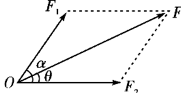
\includegraphics[width=0.3\textwidth]{511.png}
         \end{figure}
         $F=\sqrt{F_{1}^{2}+F_{2}^{2}+2F_{1}F_{2}\cos\alpha}.$
         它与$F_{2}$的夹角为$\theta$,$tan\theta=\frac{F_{1}\sin  \alpha}{F_{2}+F_{1}\cos\alpha}$.

   
      \end{itemize}
      \item 几种特殊情况的共点力的合成
      \begin{figure}[h]
         \centering
         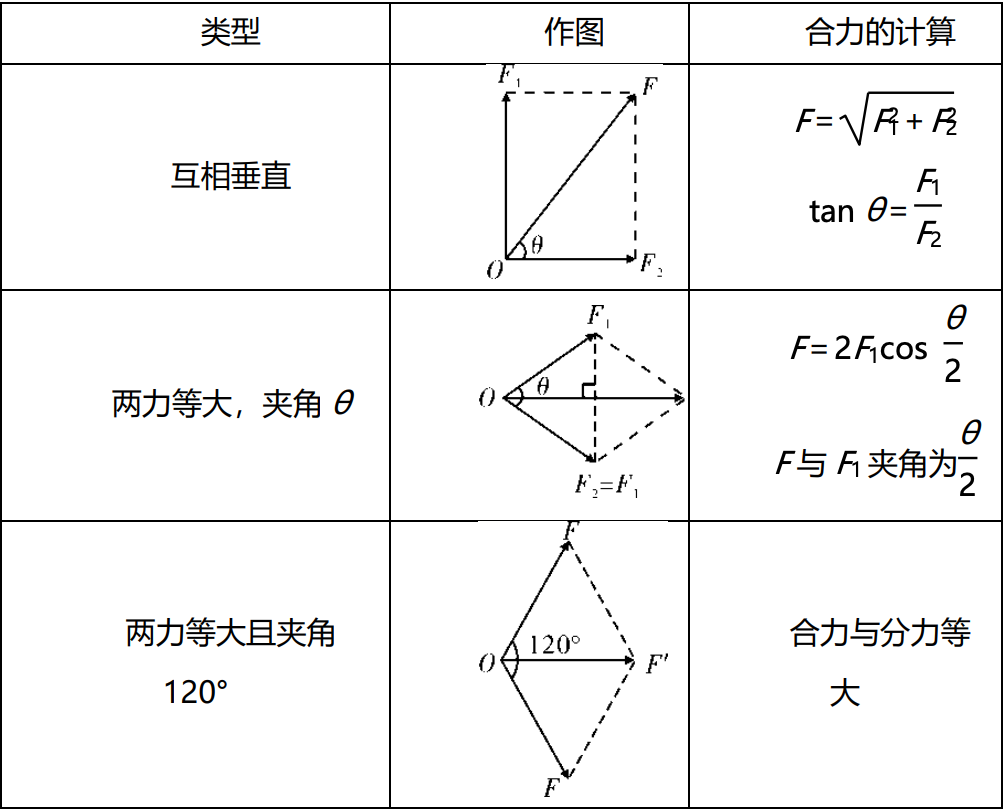
\includegraphics[width=0.7\textwidth]{512.png}
      \end{figure}

   \end{itemize}
   \begin{note}
      作图法求合力的四点要求
      \begin{itemize}
         \item 分力、合力的作用点相同,切忌弄错表示合力的对角线
         \item 分力、合力的比例要一致,力的标度要适当
         \item 虚线、实线要分清,表示分力和合力的两条邻边和对角线画成实线,
         并加上箭头,平行四边形的另两条边画成虚线
         \item 求合力时既要求出合力的大小,又要求出合力的方向
      \end{itemize}
      
   \end{note}

   

   \begin{example}
      (2017·天津卷)(多选)如图所示,
      轻质不可伸长的晾衣绳两端分别固定在竖直杆 M、N 上的 a、b 两点,
      悬挂衣服的衣架挂钩是光滑的,
      挂于绳上处于静止状态.如果只人为改变一个条件,
      当衣架静止时,下列说法正确的是( AB )
      \begin{figure}[htbp]
         \centering
         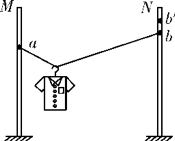
\includegraphics[width=0.3\textwidth]{513.png}
      \end{figure}
         
      A.绳的右端上移到$b^{\prime}$,绳子拉力不变
      
      B.将杆N向右移一些,绳子拉力变大

      C.绳的两端高度差越小,绳子拉力越小
      
      D.若换挂质量更大的衣服,则衣架悬挂点右移

      \begin{solution}
      oa、ob为一根绳,两端拉力相等,设绳aob长为L,
      M、N的水平距离为d,bo延长线交M于$a^{\prime}$,
      由几何知识知$a^{\prime}o=ao,\sin\theta=\frac{d}{L}$,
      由平衡条件有$2F\cos\theta=mg$,则$F=\frac{mg}{2\cos\theta}$,
      当b上移到$b^{\prime}$时,d、L不变,$\theta$不变,故F不变,
      选项A正确,C错误.将杆N向右移一些,L不变,d变大,$\theta$变大,$\cos\theta$变小,
      则F变大,选项B正确.只改变m,其他条件不变,
      则$\sin\theta$不变,$\theta$不变,衣架悬挂点不变,选项D错误. 
      \begin{figure}[htbp]
         \centering
         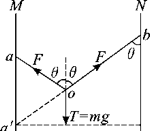
\includegraphics[width=0.3\textwidth]{514.png}
      \end{figure}
     
      \end{solution}
                  
      
   \end{example}

   \begin{note}
      \begin{itemize}
         \item 力合成时,要正确理解合力与分力的大小关系:
         合力与分力的大小关系要视情况而定,不能形成合力总大于分力的思维定式.
         \item 合力与它的分力是等效替代关系,
         在进行有关力的计算时,如果已计入了合力,就不能再计入分力;
         如果已计入了分力,就不能再计入合力.
      \end{itemize}
      
   \end{note}

   \clearpage\section{力的分解}

   \begin{itemize}
      \item 按力的作用效果分解(思路图)
      \begin{figure}[htbp]
         \centering
         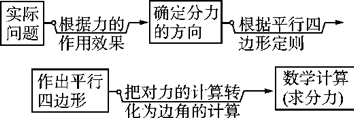
\includegraphics[width=0.5\textwidth]{521.png}
      \end{figure}

      如图所示,物体的重力G按产生的效果分解为两个分力,$F_{1}$使物体下滑,$F_{2}$使物体压紧斜面.
      \begin{figure}[htbp]
         \centering
         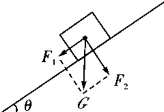
\includegraphics[width=0.2\textwidth]{522.png}
      \end{figure}

      \item 正交分解法
      \begin{itemize}
         \item 定义:将已知力按互相垂直的两个方向进行分解的方法.
         \item 建立坐标轴的原则:一般选共点力的作用点为原点,在静力学中,以少分解力和容易分解力为原则(使尽量多的力在坐标轴上);在动力学中,往往以加速度方向和垂直加速度方向为坐标轴建立坐标系.
         \item 方法:物体受到多个力$F_{1}$、$F_{2}$、$F_{3}$……作用,求合力F时,可把各力向相互垂直的x轴、y轴分解.
         \begin{figure}[htbp]
            \centering
            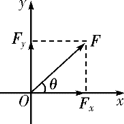
\includegraphics[width=0.1\textwidth]{523.png}
         \end{figure}
   
         \begin{itemize}
            \item x轴上的合力:$F_{x}$=$F_{x1}$+$F_{x2}$+$F_{x3}$+……
            \item y轴上的合力:$F_{y}$=$F_{y1}$+$F_{y2}$+$F_{y3}$+……
            \item 合力大小:$F=\sqrt{F_{x}^{2}+F_{y}^{2}}$
            \item 合力方向:与x轴夹角为$\theta$,则$\tan\theta=\frac{F_{y}}{F_{x}}$.

         \end{itemize}
      \end{itemize}
   \end{itemize}

   
   \begin{example}
      如图所示,光滑斜面的倾角为$\theta$,有两个相同的小球,
      分别用光滑挡板A、B挡住,挡板A沿竖直方向,挡板B垂直于斜面,
      则两挡板受到小球压力的大小之比为,
      斜面受到两个小球压力大小之比为.      
      \begin{figure}[H]
         \centering
         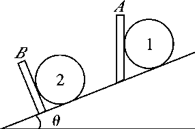
\includegraphics[width=0.2\textwidth]{524.png}
      \end{figure}

      \begin{solution}
         $1:\cos\theta;         1:\cos2\theta$
      \end{solution}

      
                  
      
   \end{example}

   \clearpage\section{“绳——杆”模型}
   \begin{itemize}
      \item “死结”与“活结”模型
      \begin{itemize}
         \item “死结”可理解为把绳子分成两段,且不可以沿绳子移动的结点.
         “死结”两侧的绳因结而变成了两根独立的绳.
         \item “活结”可理解为把绳子分成两段,且可以沿绳子移动的结点.
         “活结”一般是由绳跨过滑轮或者绳上挂一光滑挂钩而形成的.实质还是同一根绳子.
      \end{itemize}
      \item “固定杆”与“活动杆”模型
      \begin{itemize}
         \item 一般情况下,插入墙中的杆属于固定杆(如钉子).
         \item 一端用铰链相连的杆属于活动杆.
      \end{itemize}
   \end{itemize}

   \begin{note}
      “绳——杆”模型的处理方法
      \begin{itemize}
         \item 无论“死结”还是“活结”一般均以结点为研究对象进行受力分析.
         \item 由“死结”分开的两段绳子上的弹力不一定相等;
         由“活结”分开的两段绳子上弹力的大小一定相等,
         两段绳子合力的方向一定沿这两段绳子夹角的平分线.
         \item 固定杆的弹力方向不一定沿杆的方向,而活动杆的弹力方向一定沿杆的方向.
      \end{itemize}   
   \end{note}

   \begin{example}
      如图甲所示,细绳AD跨过固定的水平轻杆BC右端的定滑轮挂住一个质量为$M_{1}$的物体,
      $\angle ACB=30^{\circ}$;图乙中轻杆HG一端用铰链固定在竖直墙上,
      另一端G通过细绳EG拉住,EG与水平方向也成$30^{\circ}$,
      轻杆的G点用细绳GF拉住一个质量为$M_{2}$的物体.求:

      \begin{figure}[htbp]
         \centering
         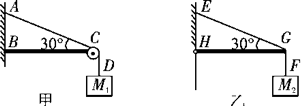
\includegraphics[width=0.3\textwidth]{531.png}
      \end{figure}
      (1)细绳 AC 段的张力 $F_{AC}$与细绳 EG 的张力 $F_{EG}$之比;

      (2)轻杆 BC 对 C 端的支持力;

      (3)轻杆 HG 对 G 端的支持力.
      \begin{solution}
         答案 

         (1)$\frac{M_{1}}{2 M_{2}}$
         (2)$M_{1} g$,方向与水平方向成$30^{\circ}$指向右上方
         (3)$\sqrt{3} \mathrm{mg}$,方向水平向右     
      \end{solution}
                  
      
   \end{example}

\chapter{受力分析共点力的平衡}
\begin{enumerate}
   \item 受力分析
   \begin{itemize}
      \item 定义:把指定物体(研究对象)在特定的物理环境中受到的所有外力都找出来,并画出受力图,这个过程就是受力分析.
      \item 受力分析的顺序:先找重力,再找接触力(弹力、摩擦力),最后分析电场力、磁场力及其他力.
      \item 受力分析的步骤
      \begin{itemize}
         \item 明确研究对象——确定分析受力的物体,研究对象可以是单个物体,也可以是多个物体的组合.
         \item 隔离物体分析——将研究对象从周围物体中隔离出来,进而分析物体受的重力、弹力、摩擦力、电磁力等,检查周围有哪些物体对它施加了力的作用
         \item 画出受力示意图——边分析边将力一一画在受力示意图上,准确标出方向
         \item 检查画出的每一个力能否找出它的施力物体,检查分析结果能否使研究对象处于题目所给的运动状态,否则,必然发生了漏力、添力或错力现象
         
      \end{itemize}
      
   \end{itemize}
   \item 共点力的平衡
   \begin{itemize}
      \item 平衡状态:物体处于静止或匀速直线运动状态
      \item 共点力的平衡条件:$F_{合}=0$或者$\left\{\begin{array}{l}{F_{x}=0} \\ {F_{y}=0}\end{array}\right.$
      \item 平衡条件的推论
      \begin{itemize}
         \item 二力平衡:如果物体在两个共点力的作用下处于平衡状态,这两个力必定大小相等、方向相反,为一对平衡力
         \item 三力平衡:如果物体在三个共点力的作用下处于平衡状态,其中任意两个力的合力一定与第三个力大小相等、方向相反
         \item 多力平衡:如果物体受多个力作用处于平衡状态,其中任何一个力与其余力的合力大小相等、方向相反
         
      \end{itemize}
   \begin{note}
      \begin{itemize}
         \item 物体在某一时刻速度为零时,物体不一定处于平衡状态
         \item 在多个共点力作用下的物体处于静止状态,如果其中一个力消失其他力保持不变,物体沿消失的力的反方向做初速度为零的匀加速直线运动
      \end{itemize}
      
   \end{note}
   \end{itemize}
   
\end{enumerate}

\clearpage\section{物体的受力分析}
\begin{note}
   整体法、隔离法在受力分析时的灵活运用
   \begin{itemize}
      \item 当所涉及的物理问题是整体与外界作用时,应用整体分析法,可使问题简单明了,而不必考虑内力的作用.
      \item 当涉及的物理问题是物体间的相互作用时,应用隔离分析法,这时系统中物体间相互作用的内力就会变为各个独立物
      体的外力.
   \end{itemize}
   
\end{note}
\begin{example}
   (2018·浙江宁波调研)如图所示,斜面小车 M 静止在光滑水平面上,一边紧贴墙壁.若再在斜面上加一物体 m,且M、m 相对静止,小车后来受力个数为( B )

   \begin{figure}[htbp]
      \centering
      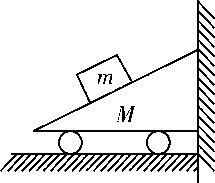
\includegraphics[width=0.2\textwidth]{611.png}
   \end{figure}
   
   A.3	
   
   B.4
   
   C.5	
   
   D.6   
   \begin{solution}
      对M和m整体,它们必受到重力和地面支持力,因小车静止,由平衡条件知墙面对小车必无作用力.以小车为研究对象,如右图所示,它受四个力:重力Mg,地面的支持力$F_{\mathrm{N} 1}$,m对它的压力$F_{\mathrm{N} 2}$和摩擦力$F_{f}$.由于m静止,可知$F_{f}$和$F_{\mathrm{N} 2}$的合力必竖直向下,故选项B正确. 
      \begin{figure}[htbp]
         \centering
         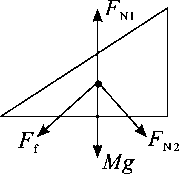
\includegraphics[width=0.2\textwidth]{612.png}
      \end{figure}
     
   \end{solution}
\end{example}


\clearpage\section{解决平衡问题常用的方法}
\begin{figure}[H]
   \centering
   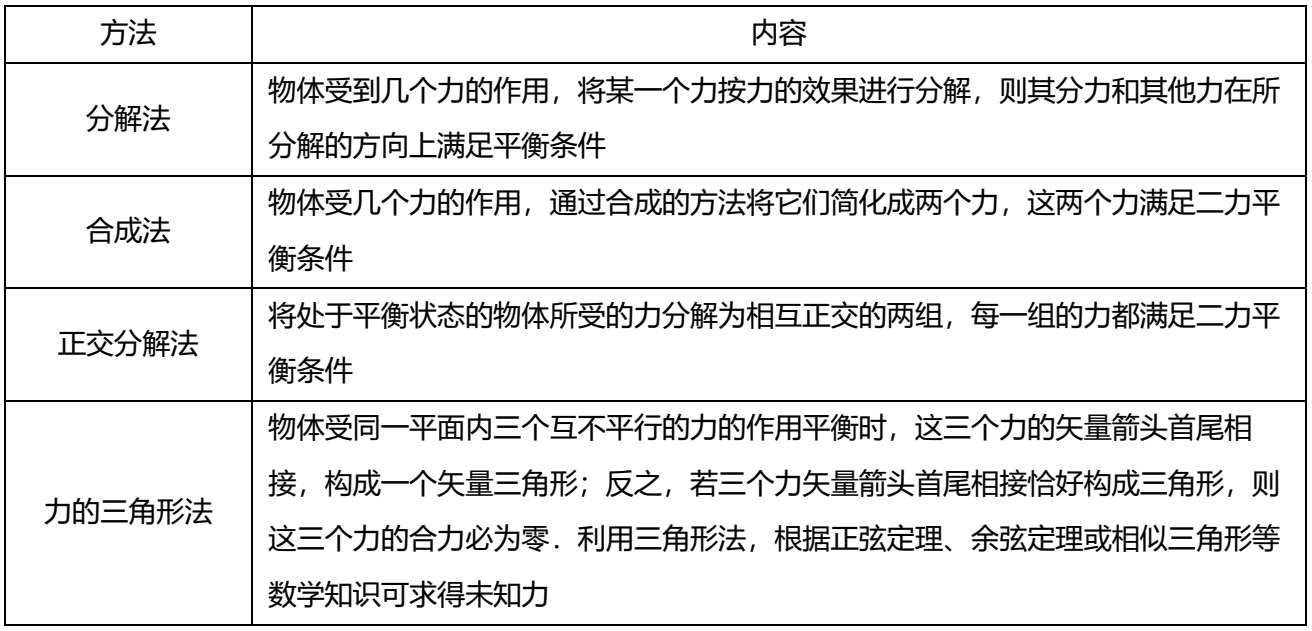
\includegraphics[width=1\textwidth]{621.png}
\end{figure}

\begin{example}
   (2018·湖南常德模拟)如图所示,重为G的均匀链条,两端用等长的轻绳连接,挂在等高的地方,轻绳与水平方向成$\theta$角.试求:

   \begin{figure}[H]
      \centering
      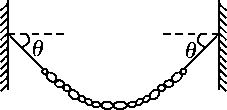
\includegraphics[width=0.2\textwidth]{622.png}
   \end{figure}
   
   (1)绳子的拉力;
   
   (2)链条在最低点的相互拉力的大小.
   \begin{solution}
      (1)$\frac{G}{2 \sin \theta}$(2)$\frac{1}{2}G\cot\theta$
     
   \end{solution}
\end{example}
\begin{note}
   应用平衡条件解题步骤
   \begin{itemize}
      \item 选取研究对象:根据题目要求,选取一个平衡体(单个物体或系统,也可以是结点)作为研究对象.
      \item 画受力示意图:对研究对象进行受力分析,画出受力示意图.
      \item 三个力直接合成或正交分解,四个及四个以上的力正交分解.
      \item 列方程求解:根据平衡条件列出平衡方程,解平衡方程,对结果进行讨论.
      
   \end{itemize}
   
\end{note}



\clearpage\section{动态平衡问题}
\begin{itemize}
   \item 动态平衡
   
   在某一物理过程中,物体或系统始终处于平衡状态,而物体或系统受到的力有一部分是变力(力的大小变或方向变或大小和方向均发生变化),这样的物理过程叫动态平衡.
   \item 基本思路
   
   化“动”为“静”,“静”中求“动”.
   \item “两种”典型方法
   \begin{figure}[htbp]
      \centering
      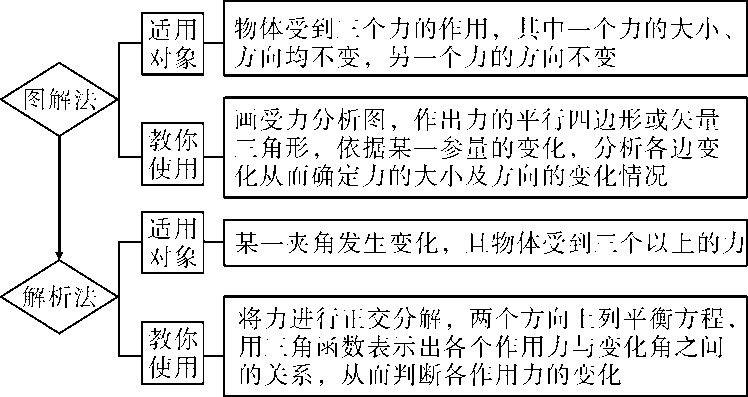
\includegraphics[width=0.8\textwidth]{631.png}
   \end{figure}
\end{itemize}
\begin{example}
   (2017·江苏南京调研)(多选)如图所示,在粗糙水平地面上放着一个截面为四分之一圆弧的柱状物体A,A的左端紧靠竖直墙,A与竖直墙之间放一光滑圆球B,已知A的圆半径为球B的半径的3倍,球B所受的重力为G,整个装置处于静止状态.设墙壁对B的压力为$F_{1}$,A对B的压力为$F_{2}$,则若把A向右移动少许后,它们仍处于静止状态,则$F_{1}$、$F_{2}$的变化情况分别是( AD )
   \begin{figure}[htbp]
      \centering
      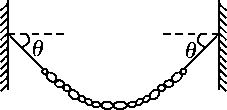
\includegraphics[width=0.2\textwidth]{622.png}
   \end{figure}
   
   A.$F_{1}$减小	

   B.$F_{1}$增大
   
   C.$F_{2}$增大	
   
   D.$F_{2}$减小   
\end{example}




\clearpage\section{平衡中的临界与极值问题}
\begin{itemize}
   \item 临界问题
   
   当某物理量变化时,会引起其他几个物理量的变化,从而使物体所处的平衡状态“恰好出现”或“恰好不出现”,在问题的描述中常用“刚好”“刚能”“恰好”等语言叙述.
   \item 极值问题
   
   平衡物体的极值,一般指在力的变化过程中的最大值和最小值问题.
   \item 解决平衡中临界与极值问题的常用方法
   \begin{itemize}
      \item 图解法:根据物体的平衡条件,作出力的矢量图,通过对物理过程的分析,利用平行四边形定则进行动态分析,确定最大值与最小值.
      \item 数学解法:通过对问题的分析,依据物体的平衡条件写出物理量之间的函数关系(或画出函数图象),用数学方法求极值(如求二次函数极值、公式极值、三角函数极值).
   \end{itemize}
\end{itemize}

\begin{example}
   (2018·云南师大附中质检)如图所示,质量为m的小球与细线连接且静止于光滑斜面上,斜面足够长,倾角$\alpha=30^{\circ}$的斜面体置于光滑水平面上,用水平力F推斜面体使斜面体缓慢地向左移动,小球沿斜面缓慢升高.当细线拉力最小时,推力F等于( A )   
   \begin{figure}[htbp]
      \centering
      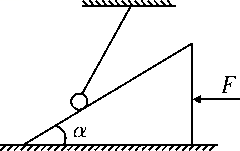
\includegraphics[width=0.2\textwidth]{641.png}
   \end{figure}
   
   A.$\frac{\sqrt{3}}{4}mg$	
   
   B.$\frac{\sqrt{3}}{2}mg$
   
   C.$mg$
   
   D.$\sqrt{3}mg$
   \begin{solution}
      小球受力动态平衡如图,可知当T平行于斜面时$T_{min}=mg\sin 30^{\circ}$,对小球和斜面体组成的系统,$F=T_{min}\cos 30^{\circ}\frac{\sqrt{3}}{4}mg$,选项A正确.
      \begin{figure}[htbp]
         \centering
         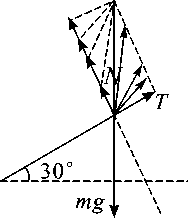
\includegraphics[width=0.2\textwidth]{642.png}
      \end{figure}
   
      
   \end{solution}   
\end{example}



\chapter{牛顿第一、第三定律}
\begin{enumerate}
   \item 牛顿第一定律
   \begin{itemize}
      \item 内容:一切物体总保持匀速直线运动状态或静止状态,直到有外力迫使它改变这种状态为止
      \item 意义
      \begin{itemize}
         \item 指出了一切物体具有惯性,因此牛顿第一定律又称惯性定律
         \item 指出力不是维持物体运动状态的原因,而是改变物体运动状态的原因,即力是产生加速度的原因
         \item 当物体不受力时,物体总保持匀速直线运动状态或静止状态
      \end{itemize}
      \item 惯性
      \begin{itemize}
         \item 定义:物体具有保持原来匀速直线运动状态或静止状态的性质
         \item 量度:质量是物体惯性大小的唯一量度,与物体的运动状态、受力情况、地理位置均无关,质量大的物体惯性大,质量小的物体惯性小
         \item 普遍性:惯性是物体的固有属性,一切物体都有惯性
      \end{itemize}
   \end{itemize}
   \item 牛顿第三定律
   \begin{itemize}
      \item 作用力和反作用力:两个物体之间的作用总是相互的,一个物体对另一个物体施加了力,另一个物体同时对这个物体也施加了力
      \item 内容:两个物体之间的作用力和反作用力总是大小相等、方向相反、作用在同一条直线上
      \item 表达式:$F=-F^{\prime}$
      \item 意义:建立了相互作用物体之间的联系及作用力与反作用力的相互依赖关系
   \end{itemize}
\end{enumerate}

\clearpage\section{牛顿第一定律的应用技巧}
\begin{itemize}
   \item 应用牛顿第一定律分析实际问题时,要把生活感受和理论问题联系起来深刻认识力和运动的关系,正确理解力不是维持物体运动状态的原因,克服生活中一些错误的直观印象,建立正确的思维习惯.
   \item 如果物体的运动状态发生改变,则物体必然受到不为零的合外力作用.因此,判断物体的运动状态是否改变,以及如何改变,应分析物体的受力情况.
\end{itemize}

\begin{example}
   伽利略创造性地把实验、假设和逻辑推理相结合的科学方法,有力地促进了人类科学认识的发展,利用如图所示的装置做如下实验:小球从左侧斜面上的O点由静止释放后沿斜面向下运动,并沿右侧斜面上升.斜面上先后铺垫三种粗糙程度逐渐降低的材料时,小球沿右侧斜面上升到的最高位置依次为1、2、3.根据三次实验结果的对比,可以得到的最直接的结论是( A )
   \begin{figure}[H]
      \centering
      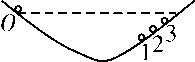
\includegraphics[width=0.2\textwidth]{711.png}
   \end{figure}
   
   A.如果斜面光滑,小球将上升到与O点等高的位置
   
   B.如果小球不受力,它将一直保持匀速运动或静止状态
   
   C.如果小球受到力的作用,它的运动状态将发生改变
   
   D.小球受到的力一定时,质量越大,它的加速度越小
   \begin{solution}
      根据题意,铺垫材料粗糙程度降低时,小球上升的最高位置升高,当斜面绝对光滑时,小球在斜面上没有能量损失,因此可以上升到与O点等高的位置,而B、C、D三个选项,从题目不能直接得出,所以选项A正确.
   
      
   \end{solution}   
\end{example}


\clearpage\section{对牛顿第三定律的理解及应用}
\begin{itemize}
   \item 相互作用力的特点:“三同、三异、三无关”.
   \begin{itemize}
      \item 三同
      \begin{itemize}
         \item 同大小
         \item 同时产生,变化,消失
         \item 同性质
      \end{itemize}
      \item 三异
      \begin{itemize}
         \item 反向
         \item 异体:作用力,反作用力作用在不同物体上
      \end{itemize}
      \item 三无关
      \begin{itemize}
         \item 与物体的种类无关
         \item 与相互作用的两物体的运动状态无关
         \item 与是否和其它物体相互作用无关
      \end{itemize}
   \end{itemize}
   \item 一对平衡力与作用力、反作用力的不同点:
   \begin{figure}[H]
      \centering
      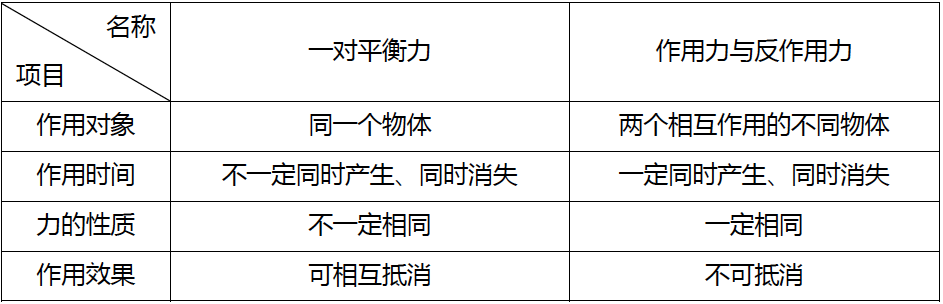
\includegraphics[width=0.8\textwidth]{721.png}
   \end{figure}

\end{itemize}

\begin{example}
   (2017·宁夏银川模拟)手拿一个锤头敲在一块玻璃上把玻璃打碎了.对于这一现象,下列说法正确的是( C )
      
   A.锤头敲玻璃的力大于玻璃对锤头的作用力,所以玻璃才碎裂
   
   B.锤头受到的力大于玻璃受到的力,只是由于锤头能够承受比玻璃更大的力才没有碎裂
   
   C.锤头和玻璃之间的作用力应该是等大的,只是由于锤头能够承受比玻璃更大的力才没有碎裂
   
   D.因为不清楚锤头和玻璃的其他受力情况,所以无法判断它们之间的相互作用力的大小关系

\end{example}

\begin{note}
   应用牛顿第三定律应注意的三个问题
   \begin{itemize}
      \item 定律中的“总是”说明对于任何物体,在任何情况下牛顿第三定律都是成立的.
      \item 作用力与反作用力虽然等大反向,但因所作用的物体不同,所产生的效果(运动效果或形变效果)往往不同.
      \item 作用力与反作用力只能是一对物体间的相互作用力,不能涉及第三个物体.
   \end{itemize}
   
\end{note}



\chapter{牛顿第二定律两类动力学问题}
\begin{enumerate}
   \item 牛顿第二定律
   \begin{itemize}
      \item 内容:物体加速度的大小跟它受到的作用力成正比,跟它的质量成反比.加速度的方向与作用力的方向相同.
      \item 表达式:$F=m a$,$F$与$a$具有瞬时对应关系.
      \item 适用范围:
      \begin{itemize}
         \item 牛顿第二定律只适用于惯性参考系(相对地面静止或做匀速直线运动的参考系).
         \item 牛顿第二定律只适用于宏观物体(相对于分子、原子)、低速运动(远小于光速)的情况.
      \end{itemize}
   \end{itemize}
   \item 动力学两类基本问题
   \begin{itemize}
      \item 动力学两类基本问题
      \begin{itemize}
         \item 已知受力情况,求物体的运动情况
         \item 已知运动情况,求物体的受力情况
      \end{itemize}
      \item 解决两类基本问题的方法:以加速度为“桥梁”,由运动学公式和牛顿运动定律列方程求解,具体逻辑关系如图所示.
   \end{itemize}
\end{enumerate}

\clearpage\section{牛顿第二定律的瞬时性}
\begin{figure}[htbp]
   \centering
   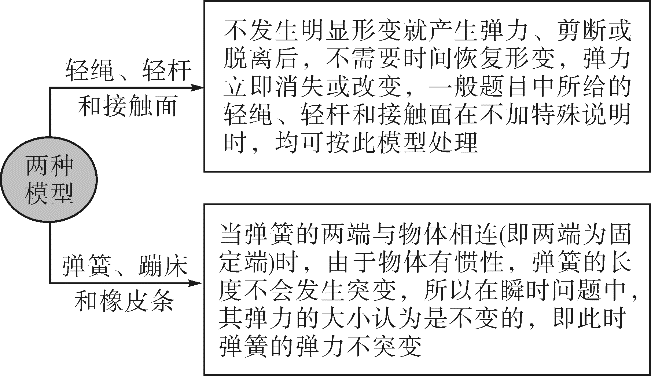
\includegraphics[width=0.6\textwidth]{811.png}
\end{figure}

\begin{example}
   (2018·广西南宁模拟)两个质量均为m的小球,用两条轻绳连接,处于平衡状态,如图所示.现突然迅速剪断轻绳OA,让小球下落,在剪断轻绳的瞬间,设小球A、B的加速度分别用$a_{1}$和$a_{2}$表示,则( A )   
   \begin{figure}[htbp]
      \centering
      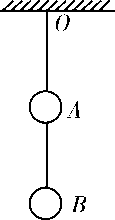
\includegraphics[width=0.1\textwidth]{812.png}
   \end{figure}

   A.$a_{1}$=g $a_{2}$=g	
   
   B.$a_{1}$=0 $a_{2}$=2g
   
   C.$a_{1}$=g $a_{2}$=0	
   
   D.$a_{1}$=2g $a_{2}$=0

   【拓展延伸1】把“轻绳”换成“轻弹簧”

   在[例1]中只将A、B间的轻绳换成轻质弹簧,其他不变,如图所示,则典例选项中正确的是( D )
   \begin{figure}[H]
      \centering
      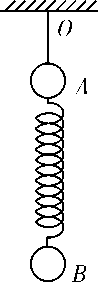
\includegraphics[width=0.1\textwidth]{813.png}
   \end{figure}
   A.$a_{1}$=g $a_{2}$=g	

   B.$a_{1}$=0 $a_{2}$=2g

   C.$a_{1}$=g $a_{2}$=0	

   D.$a_{1}$=2g $a_{2}$=0

   【拓展延伸2】改变平衡状态的呈现方式

   把【拓展延伸1】的题图放置在倾角为$\theta$=30°的光滑斜面上,如图所示系统静止时,弹簧与轻绳均平行于斜面,在轻绳被剪断的瞬间,则下列说法正确的是( B )
   \begin{figure}[htbp]
      \centering
      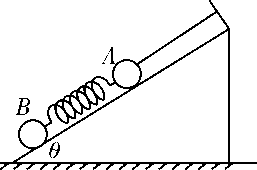
\includegraphics[width=0.2\textwidth]{814.png}
   \end{figure}
   
   A.$a_{A}$=0 $a_{B}=\dfrac {1}{2}g$

   B.$a_{A}$=g $a_{B}=0$
   
   C.$a_{A}$=g $a_{B}=g$	
   
   D.$a_{A}$=0 $a_{B}=g$

\end{example}

\begin{note}
   抓住“两关键”、遵循“四步骤”
   \begin{itemize}
      \item 分析瞬时加速度的“两个关键”
      \begin{itemize}
         \item 明确绳或线类、弹簧或橡皮条类模型的特点.
         \item 分析瞬时前、后的受力情况和运动状态.
      \end{itemize}
      \item “四个步骤”
      \begin{itemize}
         \item 第一步:分析原来物体的受力情况.
         \item 第二步:分析物体在突变时的受力情况.
         \item 第三步:由牛顿第二定律列方程.
         \item 第四步:求出瞬时加速度,并讨论其合理性.
      \end{itemize}
   \end{itemize}
   
\end{note}




\clearpage\section{动力学两类基本问题}
\begin{note}
   动力学两类基本问题的解题思路
   \begin{figure}[htbp]
      \centering
      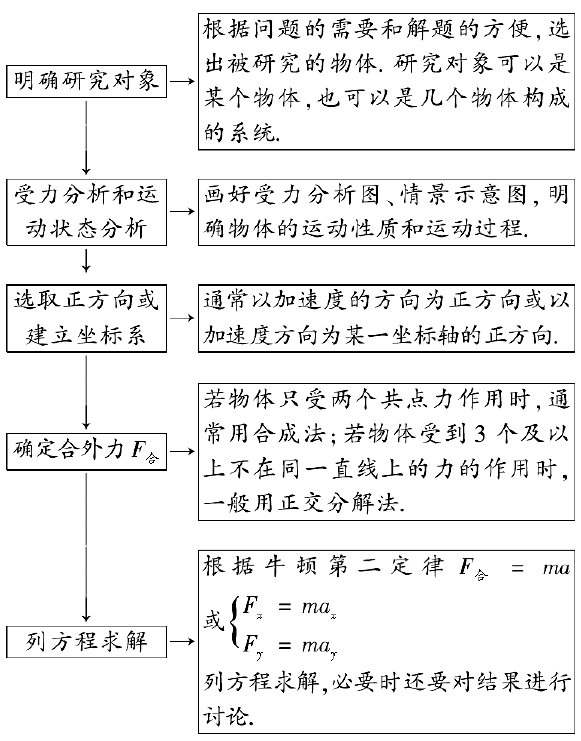
\includegraphics[width=0.7\textwidth]{821.png}
   \end{figure}
   
\end{note}

\begin{example}
   (2018·广东深圳模拟)如图所示为四旋翼无人机,它是一种能够垂直起降的小型遥控飞行器,目前得到越来越广泛的应用.      
   \begin{figure}[H]
      \centering
      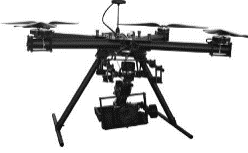
\includegraphics[width=0.3\textwidth]{822.png}
   \end{figure}
   (1)无人机在地面上从静止开始,以最大升力竖直向上起飞.求在$t=5 s$时离地面的高度$h$;
   
   (2)无人机悬停在距离地面高度$H=100 m$处,由于动力设备故障,无人机突然失去升力而坠落.求无人机坠落地面时的速度$v$;
  
   (3)在无人机坠落过程中,在遥控设备的干预下,动力设备重新启动提供向上最大升力.为保证安全着地,求飞行器从开始下落到恢复升力的最长时间$t_{1}$.
   \begin{solution}
      (1)75 m (2)40 m/s (3)$\dfrac {5\sqrt {3}}{3}s$
   \end{solution}
\end{example}

\begin{note}
   解决两类动力学问题的两个关键点
   \begin{itemize}
      \item 把握“两个分析”“一个桥梁”
      \begin{itemize}
         \item 两个分析:物体的受力情况分析和运动过程分析.
         \item 一个桥梁:加速度是联系物体运动和受力的桥梁.
      \end{itemize}
      \item 寻找多过程运动问题中各过程间的相互联系.如第一个过程的末速度就是下一个过程的初速度,画图找出各过程的位移之间的联系.
   \end{itemize}   
\end{note}



\clearpage\section{等时圆模型及其应用}
\begin{itemize}
   \item 模型特征
   \begin{figure}[htbp]
      \centering
      \includegraphics[width=0.4\textwidth]{831.png}
   \end{figure}
   \begin{itemize}
      \item 质点从竖直圆环上沿不同的光滑弦上端由静止开始滑到环的最低点所用时间相等,如图乙所示;
      \item 质点从竖直圆环上最高点沿不同的光滑弦由静止开始滑到下端所用时间相等,如图乙所示;
      \item 两个竖直圆环相切且两环的竖直直径均过切点,质点沿不同的光滑弦上端由静止开始滑到下端所用时间相等,如图丙所示.
   \end{itemize}
   \item 思维模板
   \begin{figure}[H]
      \centering
      \includegraphics[width=0.6\textwidth]{832.png}
   \end{figure}

\end{itemize}

\begin{example}
   (2017·山东济南模拟)如图所示,在倾角为$\theta$的斜面上方的A点处旋转一光滑的木板AB,B端刚好在斜面上,木板与竖直方向AC所成角度为α一小物块由A端沿木板由静止滑下,要使物块滑到斜面的时间最短,则α与$\theta$角的大小关系( B )
   
   \begin{figure}[H]
      \centering
      \includegraphics[width=0.2\textwidth]{833.png}
   \end{figure}
   A.$\alpha =\theta$	B.$\alpha =\dfrac {\theta }{2}$
   C.$\alpha =2\theta$	D.$\alpha =\dfrac {\theta }{3}$
   
\end{example}



\chapter{牛顿运动定律的综合应用}
\begin{enumerate}
   \item 超重和失重
   \begin{itemize}
      \item 实重与视重
      \begin{itemize}
         \item 实重:物体实际所受的重力,与物体的运动状态无关
         \item 视重:当物体挂在弹簧测力计下或放在水平台秤上时,弹簧测力计或台秤的示数称为视重;视重大小等于弹簧测力计所受物体的拉力或台秤所受物体的压力
      \end{itemize}
      \item 超重、失重和完全失重的比较
      
   \end{itemize}
   \item 连接体问题
   \begin{itemize}
      \item 整体法和隔离法
      \begin{itemize}
         \item 整体法:当连接体内(即系统内)各物体的加速度相同时,可以把系统内的所有物体看成一个整体,分析其受力和运动情况,运用牛顿第二定律对整体列方程求解的方法.
         \item 隔离法:当求系统内物体间相互作用的内力时,常把某个物体从系统中隔离出来,分析其受力和运动情况,再用牛顿第二定律对隔离出来的物体列方程求解的方法.
      \end{itemize}
      \item 动力学图象
      \begin{itemize}
         \item 三种图象:v-t图象、a-t图象、F-t图象
         \item 图象间的联系:加速度是联系v-t图象与F-t图象的桥梁
      \end{itemize}
   \end{itemize}
\end{enumerate}

\clearpage\section{对超重和失重的理解}
\begin{example}
   广州塔,昵称小蛮腰,总高度达600米,游客乘坐观光电梯大约一分钟就可以到达观光平台.若电梯简化成只受重力与绳索拉力,已知电梯在t=0时由静止开始上升,a-t图象如图所示,则下列相关说法正确的是( D )

   \begin{figure}[htbp]
      \centering
      \includegraphics[width=0.3\textwidth]{911.png}
   \end{figure}
   A.t=4.5 s时,电梯处于失重状态
   
   B.5~55 s时间内,绳索拉力最小
   
   C.t=59.5 s时,电梯处于超重状态
   
   D.t=60 s时,电梯速度恰好为零   
   \begin{solution}
      利用a-t图象可判断t=4.5 s时,电梯有向上的加速度,电梯处于超重状态,则选项A错误;0~5 s时间内,电梯处于超重状态,拉力>重力,5~55 s时间内,电梯处于匀速上升过程,拉力=重力,55~60 s时间内,电梯处于失重状态,拉力<重力,综上所述,选项B、C错误;因a-t图线与t轴所围的“面积”代表速度改变量,而图中横轴上方的“面积”与横轴下方的“面积”相等,则电梯的速度在t=60 s时为零,选项D正确.         
   \end{solution}
\end{example}

\begin{note}
   判断超重和失重现象的三个角度
   \begin{itemize}
      \item 从受力的角度判断
      
      当物体受向上的拉力(或支持力)大于重力时,物体处于超重状态;小于重力时处于失重状态,等于零时处于完全失重状态.
      \item 从加速度的角度判断
      
      当物体具有向上的加速度时处于超重状态,具有向下的加速度时处于失重状态,向下的加速度为重力加速度时处于完全失重状态.
      \item 从速度变化角度判断
      \begin{itemize}
         \item 物体向上加速或向下减速时,超重;
         \item 物体向下加速或向上减速时,失重.
      \end{itemize}
   \end{itemize}
   
\end{note}


\clearpage\section{动力学中的图象问题}
\begin{figure}[htbp]
   \centering
   \includegraphics[width=0.9\textwidth]{921.png}
\end{figure}

\begin{example}
   (多选)2012年11月,“歼15”舰载机在“辽宁号”航空母舰上着舰成功,图甲为利用阻拦系统让舰载机在飞行甲板上快速停止的原理示意图.飞机着舰并成功钩住阻拦索后,飞机的动力系统立即关闭,阻拦系统通过阻拦索对飞机施加一作用力,使飞机在甲板上短距离滑行后停止.某次降落,以飞机着舰为计时零点,飞机在t=0.4s时恰好钩住阻拦索中间位置,其着舰到停止的速度—时间图线如图乙所示.假如无阻拦索,飞机从着舰到停止需要的滑行距离约为1000 m.已知航母始终静止,重力加速度的大小为g,则( AC )

   \begin{figure}[H]
      \centering
      \includegraphics[width=0.5\textwidth]{922.png}
   \end{figure}
   A.从着舰到停止,飞机在甲板上滑行的距离约为无阻拦索时的
   
   B.在0.4~2.5 s时间内,阻拦索的张力几乎不随时间变化

   C.在滑行过程中,飞行员所承受的加速度大小会超过2.5g

   D.在0.4~2.5 s时间内,阻拦系统对飞机做功的功率几乎不变
   \begin{solution}
   能正确识图,并从图象中提取所需的信息,是解答此类问题的关键,本题的分析思路具有一定的代表性,逻辑流程如下:
   \begin{figure}[htbp]
      \centering
      \includegraphics[width=0.5\textwidth]{923.png}
   \end{figure}


   \end{solution}
\end{example}



\clearpage\section{连接体问题}
\begin{note}
   涉及整体法和隔离法的具体类型
   \begin{itemize}
      \item 通过滑轮和绳的连接体问题:若要求绳的拉力,一般都必须采用隔离法.绳跨过定滑轮,连接的两物体虽然加速度大小相同但方向不同,故采用隔离法.
      \item 水平面上的连接体问题:这类问题一般多是连接体(系统)中各物体保持相对静止,即具有相同的加速度.解题时,一般整体法、隔离法交替应用.
      \item 斜面体与上面物体组成的系统的问题:当物体具有沿斜面方向的加速度,而斜面体相对于地面静止时,解题时一般采用隔离法分析.
   \end{itemize}
   
\end{note}

\begin{example}
   (多选)如图所示,质量为$m_{2}$的物体,放在沿平直轨道向左行驶的车厢底板上,并用竖直细绳通过光滑的定滑轮连接质量为$m_{1}$的物体.当车向左匀加速运动时,与物体$m_{1}$相连接的绳与竖直方向成$\theta$角,$m_{2}$与车厢相对静止.则( BD )

   \begin{figure}[htbp]
      \centering
      \includegraphics[width=0.2\textwidth]{931.png}
   \end{figure}

   A.车厢的加速度为gsin $\theta$

   B.绳对物体$m_{1}$的拉力T为   
   
   C.地板对物体$m_{2}$的支持力$F_{N}$=($m_{2}$-$m_{1}$)g

   D.物体$m_{2}$所受底板的摩擦力$F_{f}$=$m_{2}$gtan $\theta$
   
   \begin{solution}
      以物体$m_{1}$为研究对象,分析受力情况如图甲所示,根据牛顿第二定律得$m_{1}$gtan $\theta$=$m_{1}$a,得a=gtan $\theta$,则车厢的加速度也为gtan $\theta$.绳对物体$m_{1}$的拉力$T=\dfrac {m_{1}g}{\cos \theta }$,故选项A错误,B正确;以物体$m_{2}$为研究对象,分析其受力情况如图乙所示,根据牛顿第二定律有$F_{N}=m_{2}g-T=m_{2}g-\dfrac {m_{1}g}{\cos \theta },F_{f}=m_{2}a=m_{2}g\tan \theta.$故选项C错误,D正确.
      
   \begin{figure}[htbp]
      \centering
      \includegraphics[width=0.2\textwidth]{932.png}
   \end{figure}


   \end{solution}
\end{example}

\begin{note}
   分析连接体问题的思路
   \begin{figure}[htbp]
      \centering
      \includegraphics[width=0.5\textwidth]{933.png}
   \end{figure}

   
\end{note}


\clearpage\section{传送带模型}
传送带模型问题包括水平传送带问题和倾斜传送带问题.
\begin{itemize}
   \item 水平传送带问题
   
   求解的关键在于对物体所受的摩擦力进行正确的分析判断.物体的速度与传送带速度相等的时刻就是物体所受摩擦力发生突变的时刻.
   \item 倾斜传送带问题
   
   求解的关键在于分析清楚物体与传送带的相对运动情况,从而确定其是否受到滑动摩擦力作用.当物体速度与传送带速度相等时,物体所受的摩擦力有可能发生突变.
\end{itemize}

\begin{example}
   (2018·山东济南重点中学联考)如图甲所示,水平传送带沿顺时针方向匀速运转.从传送带左端P先后由静止轻轻放上三个物体A、B、C,物体A经$t_{A}$=9.5 s到达传送带另一端Q,物体B经$t_{B}$=10 s到达传送带另一端Q,若释放物体时刻作为t=0时刻,分别作出三物体的v-t图象如图乙、丙、丁所示.求:

   \begin{figure}[htbp]
      \centering
      \includegraphics[width=0.6\textwidth]{941.png}
   \end{figure}

   (1)传送带的速度大小$v_{0}$;
   
   (2)PQ的长度L;
   
   (3)物体A、B、C与传送带间的动摩擦因数;
   
   (4)物体C从传送带左端P到右端Q所用的时间$t_{C}$.   
   \begin{solution}
      (1)4 m/s (2)36 m (3)0.4 0.2 0.012 5 (4)24 s      

   \end{solution}
\end{example}

\begin{note}
   滑块在水平传送带上运动常见的三个情景
   \begin{figure}[htbp]
      \centering
      \includegraphics[width=1\textwidth]{942.png}
   \end{figure}
\end{note}

\begin{example}
   如图所示,倾角为$\theta=30^{\circ}$的皮带运输机的皮带始终绷紧,且以恒定速度$v=2.5 m/s$运动,两轮相距$L_{AB}=5m$,将质量$m=1 kg$的物体无初速度地轻轻放在A处,若物体与皮带间的动摩擦因数$\mu=\frac{\sqrt{3}}{2}$(取g=10 $m/s^{2}$),物体从A运动到B共需多长时间?

   \begin{figure}[htbp]
      \centering
      \includegraphics[width=0.3\textwidth]{943.png}
   \end{figure}

   \begin{solution}
      第一阶段,物块向上匀加速运动,由牛顿第二定律有
      $\mu mg\cos\theta-mg\sin \theta=ma_{1}$,
      代入数据求得$a_{1}=2.5m/s^{2}$.
      根据匀变速直线运动规律得$v=a_{1}t_{1}$,$x_{1}=\frac{v}{2} t_{1}$,
      代入数据求得$t_{1}=1s,x_{1}=1.25 m.$
      第二阶段,由于$\mu>\tan\theta$,故物体向上匀速运动.
      $L_{AB}-x_{1}=vt_{2}$,
      $t_{2}=1.5 s.$
      总时间$t=t_{1}+t_{2}=2.5s$.

      答案 2.5 s
   \end{solution}
\end{example}

\begin{note}
   滑块在倾斜传送带上运动常见的四个情景
   
   \begin{figure}[H]
      \centering
      \includegraphics[width=0.9\textwidth]{944.png}
   \end{figure}
\end{note}



\clearpage\section{滑块——木板模型}
\begin{itemize}
   \item 模型特点:滑块(视为质点)置于木板上,滑块和木板均相对地面运动,且滑块和木板在摩擦力的相互作用下发生相对滑动.
   \item 位移关系:滑块由木板一端运动到另一端的过程中,滑块和木板同向运动时,位移之差$\Delta x=x_{1}-x_{2}=L$(板长);滑块和木板反向运动时,位移之和$\Delta x=x_{2}+x_{1}=L$.
   \begin{figure}[htbp]
      \centering
      \includegraphics[width=0.5\textwidth]{951.png}
   \end{figure}

\end{itemize}

\begin{example}
   一长木板在水平地面上运动,在$t=0$时刻将一相对于地面静止的物块轻放到木板上,以后木板运动的速度—时间图象如图所示.已知物块与木板的质量相等,物块与木板间及木板与地面间均有摩擦.物块与木板间的最大静摩擦力等于滑动摩擦力,且物块始终在木板上,取重力加速度的大小 $g=10m/s^{2}$.求:

   \begin{figure}[H]
      \centering
      \includegraphics[width=0.2\textwidth]{952.png}
   \end{figure}

   (1)物块与木板间、木板与地面间的动摩擦因数;

   (2)从$t=0$时刻到物块与木板均停止运动时,物块相对于木板的位移的大小.

   \begin{solution}
   (1)0.20 0.30 (2)1.125 m
   \end{solution}
\end{example}

\begin{note}
   “滑块——滑板”模型问题的分析思路
   \begin{figure}[H]
      \centering
      \includegraphics[width=0.6\textwidth]{953.png}
   \end{figure}
\end{note}

\chapter{曲线运动 运动的合成与分解}
\begin{enumerate}
   \item 曲线运动
   \item 运动的合成与分解
\end{enumerate}

\clearpage\section{曲线运动的条件及特点}

\clearpage\section{运动的合成与分解}

\clearpage\section{小船渡河模型}

\clearpage\section{关联速度问题}



\chapter{抛体运动的规律及应用}
\begin{enumerate}
   \item 平抛运动
   \item 斜抛运动
\end{enumerate}

\clearpage\section{平抛运动的基本规律}

\clearpage\section{与斜面关联的平抛运动}

\clearpage\section{平抛运动中的临界问题}

\clearpage\section{类平抛运动}


\chapter{圆周运动的规律及应用}
\begin{enumerate}
   \item 描述圆周运动的物理量
   \item 匀速圆周运动的向心力
   \item 离心运动
   \item 近心运动
\end{enumerate}

\clearpage\section{圆周运动中的运动学分析}

\clearpage\section{圆周运动中的动力学分析}

\clearpage\section{水平转盘中圆周运动物体的临界问题}

\clearpage\section{竖直面内圆周运动物体的临界问题}


\chapter{万有引力与航天}
\begin{enumerate}
   \item 开普勒三定律的内容、公式
   \item 万有引力定律
   \item 宇宙速度
\end{enumerate}

\clearpage\section{万有引力定律的理解与应用}
\begin{enumerate}
   \item 
\end{enumerate}

\clearpage\section{天体的质量和密度的计算}
\begin{enumerate}
   \item 
\end{enumerate}

\clearpage\section{人造卫星的运行规律}

\clearpage\section{卫星(航天器)的变轨问题及对接问题}

\clearpage\section{天体运动中的“多星”系统}

\chapter{功和功率}
\begin{enumerate}
   \item 功
   \item 功率
\end{enumerate}

\clearpage\section{恒力做功的计算}

\clearpage\section{功率的计算}

\clearpage\section{机车启动问题}

\clearpage\section{变力做功的求解方法}


\chapter{动能定理及其应用}
\begin{enumerate}
   \item 动能
   \item 动能定理
\end{enumerate}

\clearpage\section{对动能定理的理解}

\clearpage\section{动能定理的应用}

\clearpage\section{动能定理与图象结合问题}

\clearpage\section{动能定理与圆周运动结合}

\clearpage\section{用动能定理解决多过程问题}


\chapter{机械能守恒定律及其应用}
\begin{enumerate}
   \item 重力做功与重力势能的关系
   \item 弹性势能
   \item 机械能守恒定律及其应用
\end{enumerate}

\clearpage\section{机械能守恒的判断方法}

\clearpage\section{单个物体机械能守恒定律的应用}

\clearpage\section{多个物体的机械能守恒}

\clearpage\section{绳索、链条类机械能守恒问题}

\chapter{功能关系能量守恒定律}
\begin{enumerate}
   \item 功能关系
   \item 能量守恒定律
\end{enumerate}

\clearpage\section{对功能关系的理解}

\clearpage\section{摩擦力做功与能量转化}

\clearpage\section{能量转化规律的应用}


\chapter{动量定理 动量守恒定律}
\begin{enumerate}
   \item 动量、动量变化、冲量
   \item 动量定理
   \item 动量守恒定律
   \item 动量守恒定律的应用
\end{enumerate}

\clearpage\section{对功能关系的理解}

\clearpage\section{摩擦力做功与能量转化}

\clearpage\section{能量转化规律的应用}

\clearpage\section{能量转化规律的应用}
\chapter{运动的描述 匀变速直线运动的研究}
\begin{enumerate}
   \item 
\end{enumerate}

\clearpage\section{对功能关系的理解}

\clearpage\section{摩擦力做功与能量转化}

\clearpage\section{能量转化规律的应用}

\clearpage\section{能量转化规律的应用}
\chapter{运动的描述 匀变速直线运动的研究}
\begin{enumerate}
   \item 
\end{enumerate}

\clearpage\section{对功能关系的理解}

\clearpage\section{摩擦力做功与能量转化}

\clearpage\section{能量转化规律的应用}

\clearpage\section{能量转化规律的应用}
\chapter{运动的描述 匀变速直线运动的研究}
\begin{enumerate}
   \item 
\end{enumerate}

\clearpage\section{对功能关系的理解}

\clearpage\section{摩擦力做功与能量转化}

\clearpage\section{能量转化规律的应用}

\clearpage\section{能量转化规律的应用}
\chapter{运动的描述 匀变速直线运动的研究}
\begin{enumerate}
   \item 
\end{enumerate}

\clearpage\section{对功能关系的理解}

\clearpage\section{摩擦力做功与能量转化}

\clearpage\section{能量转化规律的应用}

\clearpage\section{能量转化规律的应用}
\chapter{运动的描述 匀变速直线运动的研究}
\begin{enumerate}
   \item 
\end{enumerate}

\clearpage\section{对功能关系的理解}

\clearpage\section{摩擦力做功与能量转化}

\clearpage\section{能量转化规律的应用}

\clearpage\section{能量转化规律的应用}
\chapter{运动的描述 匀变速直线运动的研究}
\begin{enumerate}
   \item 
\end{enumerate}

\clearpage\section{对功能关系的理解}

\clearpage\section{摩擦力做功与能量转化}

\clearpage\section{能量转化规律的应用}

\clearpage\section{能量转化规律的应用}

%======================================================

\nocite{*} 

\bibliography{reference}

\appendix
\chapter{物理学史}

本附录包括了

\begin{equation}
\sum_{i=1}^n x_i \equiv x_1 + x_2 +\cdots + x_n
\end{equation}



\chapter{公式图表}



\end{document}
